% Options for packages loaded elsewhere
\PassOptionsToPackage{unicode}{hyperref}
\PassOptionsToPackage{hyphens}{url}
%
\documentclass[
]{article}
\usepackage{amsmath,amssymb}
\usepackage{iftex}
\ifPDFTeX
  \usepackage[T1]{fontenc}
  \usepackage[utf8]{inputenc}
  \usepackage{textcomp} % provide euro and other symbols
\else % if luatex or xetex
  \usepackage{unicode-math} % this also loads fontspec
  \defaultfontfeatures{Scale=MatchLowercase}
  \defaultfontfeatures[\rmfamily]{Ligatures=TeX,Scale=1}
\fi
\usepackage{lmodern}
\ifPDFTeX\else
  % xetex/luatex font selection
\fi
% Use upquote if available, for straight quotes in verbatim environments
\IfFileExists{upquote.sty}{\usepackage{upquote}}{}
\IfFileExists{microtype.sty}{% use microtype if available
  \usepackage[]{microtype}
  \UseMicrotypeSet[protrusion]{basicmath} % disable protrusion for tt fonts
}{}
\makeatletter
\@ifundefined{KOMAClassName}{% if non-KOMA class
  \IfFileExists{parskip.sty}{%
    \usepackage{parskip}
  }{% else
    \setlength{\parindent}{0pt}
    \setlength{\parskip}{6pt plus 2pt minus 1pt}}
}{% if KOMA class
  \KOMAoptions{parskip=half}}
\makeatother
\usepackage{xcolor}
\usepackage{color}
\usepackage{fancyvrb}
\newcommand{\VerbBar}{|}
\newcommand{\VERB}{\Verb[commandchars=\\\{\}]}
\DefineVerbatimEnvironment{Highlighting}{Verbatim}{commandchars=\\\{\}}
% Add ',fontsize=\small' for more characters per line
\usepackage{framed}
\definecolor{shadecolor}{RGB}{248,248,248}
\newenvironment{Shaded}{\begin{snugshade}}{\end{snugshade}}
\newcommand{\AlertTok}[1]{\textcolor[rgb]{0.94,0.16,0.16}{#1}}
\newcommand{\AnnotationTok}[1]{\textcolor[rgb]{0.56,0.35,0.01}{\textbf{\textit{#1}}}}
\newcommand{\AttributeTok}[1]{\textcolor[rgb]{0.13,0.29,0.53}{#1}}
\newcommand{\BaseNTok}[1]{\textcolor[rgb]{0.00,0.00,0.81}{#1}}
\newcommand{\BuiltInTok}[1]{#1}
\newcommand{\CharTok}[1]{\textcolor[rgb]{0.31,0.60,0.02}{#1}}
\newcommand{\CommentTok}[1]{\textcolor[rgb]{0.56,0.35,0.01}{\textit{#1}}}
\newcommand{\CommentVarTok}[1]{\textcolor[rgb]{0.56,0.35,0.01}{\textbf{\textit{#1}}}}
\newcommand{\ConstantTok}[1]{\textcolor[rgb]{0.56,0.35,0.01}{#1}}
\newcommand{\ControlFlowTok}[1]{\textcolor[rgb]{0.13,0.29,0.53}{\textbf{#1}}}
\newcommand{\DataTypeTok}[1]{\textcolor[rgb]{0.13,0.29,0.53}{#1}}
\newcommand{\DecValTok}[1]{\textcolor[rgb]{0.00,0.00,0.81}{#1}}
\newcommand{\DocumentationTok}[1]{\textcolor[rgb]{0.56,0.35,0.01}{\textbf{\textit{#1}}}}
\newcommand{\ErrorTok}[1]{\textcolor[rgb]{0.64,0.00,0.00}{\textbf{#1}}}
\newcommand{\ExtensionTok}[1]{#1}
\newcommand{\FloatTok}[1]{\textcolor[rgb]{0.00,0.00,0.81}{#1}}
\newcommand{\FunctionTok}[1]{\textcolor[rgb]{0.13,0.29,0.53}{\textbf{#1}}}
\newcommand{\ImportTok}[1]{#1}
\newcommand{\InformationTok}[1]{\textcolor[rgb]{0.56,0.35,0.01}{\textbf{\textit{#1}}}}
\newcommand{\KeywordTok}[1]{\textcolor[rgb]{0.13,0.29,0.53}{\textbf{#1}}}
\newcommand{\NormalTok}[1]{#1}
\newcommand{\OperatorTok}[1]{\textcolor[rgb]{0.81,0.36,0.00}{\textbf{#1}}}
\newcommand{\OtherTok}[1]{\textcolor[rgb]{0.56,0.35,0.01}{#1}}
\newcommand{\PreprocessorTok}[1]{\textcolor[rgb]{0.56,0.35,0.01}{\textit{#1}}}
\newcommand{\RegionMarkerTok}[1]{#1}
\newcommand{\SpecialCharTok}[1]{\textcolor[rgb]{0.81,0.36,0.00}{\textbf{#1}}}
\newcommand{\SpecialStringTok}[1]{\textcolor[rgb]{0.31,0.60,0.02}{#1}}
\newcommand{\StringTok}[1]{\textcolor[rgb]{0.31,0.60,0.02}{#1}}
\newcommand{\VariableTok}[1]{\textcolor[rgb]{0.00,0.00,0.00}{#1}}
\newcommand{\VerbatimStringTok}[1]{\textcolor[rgb]{0.31,0.60,0.02}{#1}}
\newcommand{\WarningTok}[1]{\textcolor[rgb]{0.56,0.35,0.01}{\textbf{\textit{#1}}}}
\usepackage{graphicx}
\makeatletter
\def\maxwidth{\ifdim\Gin@nat@width>\linewidth\linewidth\else\Gin@nat@width\fi}
\def\maxheight{\ifdim\Gin@nat@height>\textheight\textheight\else\Gin@nat@height\fi}
\makeatother
% Scale images if necessary, so that they will not overflow the page
% margins by default, and it is still possible to overwrite the defaults
% using explicit options in \includegraphics[width, height, ...]{}
\setkeys{Gin}{width=\maxwidth,height=\maxheight,keepaspectratio}
% Set default figure placement to htbp
\makeatletter
\def\fps@figure{htbp}
\makeatother
\setlength{\emergencystretch}{3em} % prevent overfull lines
\providecommand{\tightlist}{%
  \setlength{\itemsep}{0pt}\setlength{\parskip}{0pt}}
\setcounter{secnumdepth}{5}
\usepackage{fancyhdr}
\usepackage{caption}
\captionsetup[table]{justification=raggedright, singlelinecheck=false} % Left-justified table captions
\usepackage[margin=1in]{geometry} % Adjusts page margins to prevent text overflow
\setlength{\parindent}{0pt} % Removes indentation on the title page for alignment
\pagenumbering{gobble} % Hides page number on title page
\usepackage[none]{hyphenat}
\setlength{\emergencystretch}{3em}
\usepackage{ragged2e}
\justifying
\usepackage{booktabs}
\usepackage{longtable}
\usepackage{array}
\usepackage{multirow}
\usepackage{wrapfig}
\usepackage{float}
\usepackage{colortbl}
\usepackage{pdflscape}
\usepackage{tabu}
\usepackage{threeparttable}
\usepackage{threeparttablex}
\usepackage[normalem]{ulem}
\usepackage{makecell}
\usepackage{xcolor}
\ifLuaTeX
  \usepackage{selnolig}  % disable illegal ligatures
\fi
\IfFileExists{bookmark.sty}{\usepackage{bookmark}}{\usepackage{hyperref}}
\IfFileExists{xurl.sty}{\usepackage{xurl}}{} % add URL line breaks if available
\urlstyle{same}
\hypersetup{
  pdftitle={``Navigating the Digital Divide: The Role of ICT in Enhancing Educational Outcomes in Thailand''},
  hidelinks,
  pdfcreator={LaTeX via pandoc}}

\title{``Navigating the Digital Divide: The Role of ICT in Enhancing
Educational Outcomes in Thailand''}
\author{Leigh Pearson, Ph.D.~Candidate\\
School of Global Studies, Thammasat University\\
International College, Mahidol University\\
\href{mailto:leigh.pea@mahidol.edu}{\nolinkurl{leigh.pea@mahidol.edu}}}
\date{Last Updated: 15-02-2025}

\begin{document}
\maketitle

\textbf{Note}: The analyses and findings presented in this document are
part of an ongoing PhD research project focused on ICT use in education
within Thailand. These results represent preliminary findings and are
intended to fulfill initial publication requirements. The complete
research project, which includes further analyses and comprehensive
conclusions, is described in full within the
\href{https://github.com/justleigh/PhD-ICT-Education-Analysis}{PhD-ICT-Education-Analysis
repository}. As the project progresses, additional insights and updates
will be incorporated to provide a complete view of ICT's role in
educational outcomes.

\pagenumbering{arabic}

\newpage
\tableofcontents

\newpage

\hypertarget{introduction}{%
\section{Introduction}\label{introduction}}

In an era where Information and Communications Technology (ICT) has
become a cornerstone of global development, the role of ICT in education
is especially crucial. Countries around the world are leveraging digital
technologies to enhance learning, improve equity, and drive innovation
in education.

The Thai education system has been a topic of concern for policymakers,
educators, and parents for many years, and yet Thailand has made
significant, often under-appreciated progress towards realising its
aspiration of transforming into a high-income, knowledge-based economy.
The country's vision details ambitious goals to upgrade the quality of
education and provide its young people with 21st-century skills, as laid
out by the National Strategy Committee (NSC, 2019) in its twenty-year
National Strategy (2017--2036) and by the Office of the National
Economic and Social Development Council (ONESDC, 2022) in its 12th and
13th National Economic and Social Development Plan (2017-2021 \&
2023-2027).

Despite these efforts, Thai students' performance on international
benchmarks has consistently lagged behind regional and global peers. For
instance, the average scores for the five O-NET subjects have
consistently fallen below 50 percent (National Institute of Educational
Testing Service, 2021), PISA scores have been in an increasingly steep
decline since 2012 in all three skills, particularly reading (OECD,
2023), and Thailand ranks 101st out of 113 participating countries for
English proficiency (English First, 2023).

This discrepancy points to a critical gap between policy aspirations and
on-the-ground realities. While there has been substantial progress in
terms of ICT infrastructure and resources, the impact of these
advancements on actual learning outcomes remains unclear. Furthermore,
disparities in ICT access between urban and rural students, known as the
`first' digital divide, along with the `second' digital divide, which
reflects inequalities in ICT usage, together intensify educational
inequalities, particularly affecting marginalized and disadvantaged
students (Ma \& Cheng, 2022).

This research, situated at the intersection of national policy and
educational outcomes, aims to explore how ICT integration within Thai
schools influences learning outcomes and equity. Using a combination of
the PISA ICT Framework (OECD, 2019) and the Multi-Level Framework of
Technology Acceptance and Use (MLFTAU; Venkatesh et al., 2016), this
study will provide a nuanced understanding of both structural and
behavioral factors that shape ICT use in educational settings.

Through an analysis of PISA datasets spanning multiple years and
complemented by data from key national agencies, such as the National
Statistical Office of Thailand, the Equitable Education Fund (EEF), and
the Office of Basic Education Commission (OBEC), this research will
assess the effectiveness of ICT in enhancing educational outcomes.
Special attention will be given to how ICT impacts underprivileged
students, who are often left behind in national efforts to digitize
education.

By examining Thailand's experience, this research will contribute
valuable insights to the global discourse on the role of technology in
education, particularly in developing countries facing similar digital
and educational challenges.

\hypertarget{research-questions}{%
\section{Research Questions}\label{research-questions}}

\begin{enumerate}
\def\labelenumi{\arabic{enumi}.}
\item
  How does in-classroom use of ICT affect student learning outcomes in
  Thailand?
\item
  What role does ICT use outside of the classroom play in the learning
  outcomes of Thai students?
\item
  How do contextual factors, such as socio-economic status and access to
  technology, moderate the relationship between ICT use and educational
  performance?
\end{enumerate}

\hypertarget{utilization-of-conceptual-and-theoretical-frameworks}{%
\section{Utilization of Conceptual and Theoretical
Frameworks}\label{utilization-of-conceptual-and-theoretical-frameworks}}

This study employs three complementary frameworks: the PISA
Questionnaire Framework, the PISA ICT Framework, and the Multi-Level
Framework of Technology Acceptance and Use (MLFTAU). Together, these
frameworks provide a comprehensive foundation for analyzing the
systemic, behavioral, and outcome-driven factors influencing ICT
integration in education.

\textbf{The PISA Questionnaire Framework}

The PISA Questionnaire Framework serves as a holistic tool for
understanding educational systems through its 21 modules, which address
a wide range of student, school, and system-level factors. This
overarching framework provides the foundation for assessing contextual
inputs and outputs, offering internationally validated benchmarks for
evaluating educational outcomes.

\textbf{The PISA ICT Framework}

The PISA ICT Framework, a specialized subset of the PISA Questionnaire
Framework, focuses specifically on ICT access, use, and its impacts. It
is divided into two distinct components:

\begin{itemize}
\item
  In-School ICT Framework: Examines ICT resources, infrastructure, and
  practices within schools, such as the availability of technology,
  teacher guidance, and classroom integration.
\item
  Outside-the-Classroom ICT Framework: Evaluates ICT use and access
  beyond school environments, including students' home access to digital
  tools and their independent use of technology for learning and
  leisure.
\end{itemize}

This dual perspective enables a systematic analysis of ICT's role both
within formal learning environments and in students' broader educational
ecosystems.

\textbf{The Multi-Level Framework of Technology Acceptance and Use
(MLFTAU)}

The MLFTAU framework complements the PISA frameworks by addressing the
behavioral and psychological factors driving ICT adoption and use. It
evaluates how individual, group, and organizational factors influence
the acceptance and effective use of ICT. Key constructs such as
performance expectancy, facilitating conditions, and social influence
help analyze the motivations and barriers to ICT engagement.

By integrating these frameworks, this study bridges the systemic factors
(captured by the PISA Questionnaire and ICT frameworks) with behavioral
constructs (captured by MLFTAU) to evaluate how ICT access, use, and
facilitating conditions influence educational outcomes in Thailand. The
inclusion of the Output domain---measuring cognitive learning outcomes,
ICT competencies, and well-being---ensures a holistic analysis of both
inputs and impacts.

\hypertarget{pisa-questionnaire-framework}{%
\subsection{PISA Questionnaire
Framework}\label{pisa-questionnaire-framework}}

The PISA Questionnaire Framework, developed by the OECD, provides a
comprehensive structure for evaluating the contextual, systemic, and
individual factors that influence student learning outcomes. The PISA
Questionnaire Framework is designed to complement the PISA cognitive
assessments in reading, mathematics, and science literacy. While the
cognitive assessments measure student performance on standardized tasks,
the questionnaire modules provide the contextual information needed to
explain variations in student outcomes and analyze relationships between
educational inputs, processes, and results.

This dual approach ensures a comprehensive evaluation of learning
systems, enabling researchers to identify the conditions that enable or
constrain educational achievement. The framework consists of 21 modules
covering a wide range of variables, such as socio-economic background,
family environment, school resources, and teaching practices. These
modules complement the PISA assessment results by offering deeper
insights into the factors that enable or constrain educational
achievement.

\textbf{International Comparability and Standardization}

A key strength of the PISA Questionnaire Framework is its standardized
design, which ensures cross-country comparability. By collecting
consistent data across diverse educational systems, PISA enables
researchers to analyze global trends in educational performance and
equity and benchmark country-specific findings, such as ICT use in
Thailand, against international standards. For this study, the
international comparability of PISA data adds significant value,
situating Thailand's educational outcomes within a global context and
highlighting areas for improvement.

\textbf{Origins of the CIPO Framework}

The PISA Questionnaire Framework was inspired by the CIPO model
(Context, Input, Process, and Output), a foundational structure for
evaluating educational systems. The CIPO model organizes variables into
four components:

\begin{itemize}
\item
  \textbf{Context}: The socio-economic, cultural, and systemic
  environment surrounding education.
\item
  \textbf{Input}: Resources, teacher training, student characteristics,
  and infrastructure.
\item
  \textbf{Process}: Practices, methods, and pedagogical approaches
  within and beyond classrooms.
\item
  \textbf{Output}: Measurable outcomes, including academic performance,
  competencies, and well-being.
\end{itemize}

PISA now intentionally avoids labeling variables as Context, Input,
Process, or Output in recognition of the fact that many variables can
serve multiple functions depending on the context or research focus. For
example, a student's confidence in a subject can be analyzed both as an
Input (for example, a personal characteristic influencing learning
behaviours and outcomes) and/or an Output (for example, a result of
prior teaching practices and learning experiences).

Nevertheless, in this study, the CIPO domains are applied to the PISA
Questionnaire Framework with the understanding that variables can align
with multiple domains simultaneously. This flexible approach allows for
a more nuanced analysis, offering insights into where in the educational
process learning is supported or constrained.

\textbf{Scope and Focus of the PISA Questionnaire Framework}

While the PISA Questionnaire Framework is not specifically focused on
ICT, it provides a broader understanding of the educational landscape in
which ICT access, use, and impacts can be analyzed. By offering a
systemic view of students' environments---both in and outside
school---it enables researchers to:

\begin{itemize}
\item
  Examine ICT use within the broader contexts of socio-economic factors,
  school resources, and teaching practices.
\item
  Identify interacting variables that may facilitate or hinder ICT
  adoption and its effectiveness.
\end{itemize}

In this study, the broader scope of the PISA Questionnaire Framework
serves as a foundation for understanding the conditions under which ICT
is integrated into education, both systemically and behaviorally.

\textbf{Rationale for Including CIPO Domains}

For this study, the CIPO domains (Context, Input, Process, Output) have
been applied to the PISA Questionnaire Framework to facilitate a more
structured and insightful analysis. By organizing variables within the
CIPO structure, this study seeks to identify:

\begin{enumerate}
\def\labelenumi{\arabic{enumi}.}
\item
  Where in the educational process (context, input, or process) learning
  is enabled or constrained.
\item
  How specific variables can interact across domains to influence
  educational outcomes.
\end{enumerate}

It is important to note that variables may be assigned to multiple
domains where relevant. For instance, a variable like ``ICT
familiarity'' may reflect both:

\begin{itemize}
\item
  \textbf{Input}: As a measure of students' prior access and exposure to
  technology.
\item
  \textbf{Process}: As an indicator of how ICT is integrated into
  teaching and learning.
\end{itemize}

This multi-categorization approach allows for a more nuanced
understanding of the role of ICT in education, reflecting the
complexities of real-world learning environments.

\textbf{Structure of the PISA Questionnaire Framework}

The PISA Questionnaire Framework's 21 modules are grouped under broad
thematic areas, capturing critical aspects of students' learning
environments and experiences. The following table presents key modules
and their alignment with potential CIPO domains:

\begin{longtable}[l]{>{\raggedright\arraybackslash}p{1.5cm}>{\raggedright\arraybackslash}p{3.5cm}>{\raggedright\arraybackslash}p{5cm}>{\raggedright\arraybackslash}p{5cm}}
\caption{\label{tab:pisa_questionnaire_framework}Key Constructs/Modules of the PISA Questionnaire Framework}\\
\toprule
Domain & Module.Construct & Definition & Relevance\\
\midrule
Context & 1. Basic Demographics & Includes characteristics like students' age, gender, and grade level. & Provides foundational data to understand disparities in performance and participation.\\
 & 2. Economic, Social, and Cultural Status (ESCS) & Measures the economic, social, and cultural position of students and their families. & Essential for assessing equity and access to resources and opportunities.\\
 & 4. Migration and Language Exposure & Examines students' linguistic and cultural backgrounds. & Helps explain performance gaps related to linguistic diversity and cultural differences.\\
 & 6. School Culture and Climate & Explores the social and emotional environment of the school. & Provides insights into how school climate affects student engagement and learning outcomes.\\
 & 11. School Type and Infrastructure & Captures characteristics of the school, such as facilities and technology. & Highlights disparities in resources that affect engagement and learning.\\
\addlinespace
 & 12. Selection and Enrolment & Describes how students are admitted to schools. & Explains systemic inequities related to admission policies and tracking systems.\\
 & 21. Global Crises & Explores the effects of global challenges, such as pandemics or environmental crises, on education. & Provides a broader contextual understanding of external factors influencing school environments and student learning.\\
Input & 5. PISA Preparation and Effort & Covers students’ effort, time, and strategies related to PISA preparation. & Reflects motivation and cognitive engagement, key for interpreting PISA results.\\
 & 7. Subject-Specific Beliefs, Attitudes, Feelings, and Behaviours & Explores students' self-concept, enjoyment, and attitudes toward specific subjects. & Highlights the role of attitudes and interest in shaping domain-specific outcomes.\\
 & 9. Health and Well-Being & Assesses students' physical and mental health as well as their well-being. & Highlights the impact of health on educational outcomes and student engagement.\\
\addlinespace
 & 10. Out-of-School Experiences & Captures extracurricular activities and responsibilities outside school. & Shows how non-school experiences impact engagement and overall outcomes.\\
 & 13. School Autonomy & Examines the extent of school-level decision-making and autonomy. & Explores how autonomy in resource allocation and curriculum design impacts school functioning.\\
 & 14. Organisation of Student Learning at School & Captures how learning is structured at school (e.g., classroom setup, curriculum). & Highlights the organizational factors influencing teaching and learning.\\
 & 17. Teacher Qualification, Training, and Professional Development & Captures the qualifications and training of teachers. & Explains how teacher preparedness impacts classroom instruction and student outcomes.\\
 & 19. Parental/Guardian Involvement and Support & Assesses the role of parents/guardians in supporting students' education. & Correlates parental involvement with better academic outcomes and emotional well-being.\\
\addlinespace
Process & 15. Exposure to Mathematics Content & Assesses students' opportunities to engage with formal and applied mathematics tasks and reasoning activities. & Offers insight into the quality and quantity of mathematics instruction, linking teaching practices to student outcomes.\\
 & 16. Mathematics Teacher Behaviours & Captures teacher practices and interactions with students, including instructional approaches and support. & Provides data on effective teaching practices that enhance student learning and participation in mathematics.\\
 & 18. Assessment, Evaluation, and Accountability & Covers school-level practices related to student assessment and the use of achievement data for accountability purposes. & Explores how assessment and feedback practices influence learning and instructional improvement.\\
Output & 3. Educational Pathways and Post-Secondary Aspirations & Explores students’ plans for further education, career aspirations, and how they perceive their future opportunities. & Reflects the outcomes of educational experiences and their influence on students’ life goals and trajectories.\\
 & 8. General Social and Emotional Characteristics & Measures students’ interpersonal and intrapersonal skills, such as emotional regulation, resilience, and empathy. & Explores how these characteristics influence academic outcomes, well-being, and broader life outcomes.\\
\addlinespace
 & 9. Health and Well-Being & Assesses students’ physical, mental, and emotional health, as well as their overall life satisfaction. & Highlights the impact of health and well-being on students' ability to succeed in school and beyond.\\
 & 20. Creative Thinking & Captures students’ ability to generate, evaluate, and refine ideas creatively in a variety of contexts. & Evaluates creativity as a critical 21st-century skill linked to problem-solving and academic success.\\
\bottomrule
\end{longtable}

The PISA Questionnaire Framework, when analyzed using the CIPO
structure, allows this study to:

\begin{enumerate}
\def\labelenumi{\arabic{enumi}.}
\item
  Assess the systemic factors influencing ICT access and use (e.g.,
  policies, resources, socio-economic environment).
\item
  Examine the inputs and processes that enable or constrain ICT
  integration in schools and homes.
\item
  Identify outcomes (e.g., academic performance, ICT competencies,
  well-being) as measures of ICT effectiveness.
\end{enumerate}

By applying the CIPO domains flexibly, this study embraces the
complexity of educational processes, acknowledging that variables can
influence multiple stages of learning. The broader scope of the PISA
Questionnaire Framework ensures that ICT use is analyzed within its
wider educational context, enhancing the depth and breadth of the
insights gained.

The PISA Questionnaire Framework provides a robust foundation for
evaluating the systemic and contextual factors shaping ICT access and
use. While its scope extends beyond ICT, it offers essential insights
into the educational environment in which ICT operates. By integrating
the CIPO domains into the analysis, this study enables a structured yet
flexible approach to identifying the factors that help or hinder
learning outcomes.

\hypertarget{pisa-ict-framework}{%
\subsection{PISA ICT Framework}\label{pisa-ict-framework}}

The PISA ICT Framework, developed by the OECD, was introduced for the
first time in the 2022 PISA assessment to specifically evaluate the role
and impact of Information and Communication Technology (ICT) in
education. Building on the foundations of the CIPO model (Context,
Input, Process, and Output), the framework provides a structured
approach for analyzing ICT access, use, and outcomes across both school
and home environments.

The PISA ICT Framework reflects the increasing importance of ICT in
modern education, recognizing its role in enhancing student learning
outcomes, digital competencies, and engagement. To achieve a
comprehensive understanding, the framework is divided into two
complementary components:

\begin{enumerate}
\def\labelenumi{\arabic{enumi}.}
\item
  In-School ICT Framework: Examines ICT-related resources, processes,
  and pedagogical practices within formal school environments.
\item
  Outside-the-Classroom ICT Framework: Evaluates ICT access, use, and
  impacts in students' home environments and broader educational
  ecosystems.
\end{enumerate}

Together, these components offer a systemic and layered analysis of
ICT's role in enhancing student learning outcomes, engagement, and
digital competencies.

\textbf{Origins of the PISA ICT Framework}

Similar to the PISA Questionnaire Framework, this new ICT framework has
also been adapted from the older CIPO model, which is structured around
four components:

\textbf{- Context:} The broader environment in which the educational
system operates, including socio-economic, policy, and infrastructure
factors that shape ICT access and use.

\textbf{- Input:} Resources and support systems provided to schools,
such as funding, ICT infrastructure, and training for teachers, as well
as the personal characteristics of students and teachers.

\textbf{- Process:} The methods, pedagogies, and practices through which
ICT is implemented within educational settings, both in-class and
outside-the-classroom.

\textbf{- Output:} The measurable outcomes of ICT use, including
academic performance, student engagement, and digital skills.

This structured approach ensures that ICT integration is examined
holistically, considering both its systemic context and practical
implementation.

\textbf{Structure of the PISA Questionnaire Frameworks}

The PISA ICT Framework comprises two key components that reflect the
different environments where ICT access, use, and outcomes are observed:
in-school and outside-the-classroom. These components allow for a
systematic analysis of ICT integration across formal educational
settings and informal learning environments, ensuring a holistic
understanding of how ICT supports or hinders student outcomes.

To operationalize this analysis, each component is mapped onto relevant
constructs that align with the CIPO model domains (Context, Input,
Process, and Output). The tables below outline the key constructs and
their relevance for both in-school and outside-the-classroom ICT use.

\textbf{In-School ICT Constructs}

The in-school ICT framework focuses on the availability, integration,
and support of ICT resources within formal school environments. This
includes variables related to infrastructure, teacher training, and
pedagogical practices that shape ICT use in classrooms. Table 1 presents
the relevant constructs, organized within the CIPO structure, to provide
a clear framework for analyzing ICT use in schools.

\begin{longtable}[l]{>{\raggedright\arraybackslash}p{1.5cm}>{\raggedright\arraybackslash}p{3.5cm}>{\raggedright\arraybackslash}p{5cm}>{\raggedright\arraybackslash}p{5cm}}
\caption{\label{tab:in_school_constructs}Key Constructs of the PISA ICT Framework - In-School Dimension}\\
\toprule
Dimension & Construct & Definition & Relevance\\
\midrule
Context & General School Environment & Overall school characteristics that influence ICT adoption, including leadership and culture. & Highlights the broader school environment that affects ICT integration and digital education strategies.\\
 & School ICT Infrastructure & Availability, accessibility, and quality of ICT tools, internet connectivity, and digital devices. & Measures schools' readiness to adopt technology and provide equitable access to ICT tools for students.\\
 & Teacher ICT Competencies & Teachers' skills, confidence, and preparedness to integrate ICT into teaching practices. & Reflects the importance of teacher capabilities in achieving successful ICT integration for learning outcomes.\\
 & ICT-Related Policies and Guidelines & Formalized rules and policies governing the use of ICT in schools. & Demonstrates the role of structured policies in ensuring ICT is used effectively and equitably in education.\\
 & Teachers’ and Principals’ Attitudes & Perceptions, beliefs, and attitudes toward the value of ICT for teaching and learning. & Explores the extent to which attitudes influence ICT adoption and pedagogical practices in schools.\\
\addlinespace
 & Socio-Economic and Cultural Factors & Socio-economic and cultural background of the school influencing ICT access and use. & Highlights equity issues and contextual differences affecting ICT integration at the school level.\\
Input & Hardware and Software Availability & Availability of computers, tablets, internet connectivity, and software for teaching and learning. & Captures resource availability that determines ICT integration in the classroom.\\
 & Digital Learning Resources & Access to online content, intelligent tutoring systems, and other educational technologies. & Reflects the quality and range of ICT-based tools supporting teaching and learning in schools.\\
 & Technical Support for ICT Use & Availability of ICT coordinators, troubleshooting services, and technical assistance. & Ensures teachers and students have the necessary technical support to facilitate ICT-based education.\\
 & Teacher Professional Development & Opportunities for teachers to receive training on ICT integration and usage. & Emphasizes the role of continuous professional development in improving teacher ICT competencies.\\
\addlinespace
 & Incentives and Support for ICT Use & Motivational factors such as rewards, recognition, or reduced workloads to encourage ICT use. & Highlights incentives as facilitators for teachers to embrace ICT tools in pedagogy.\\
Process & Students’ Use of ICT & The extent to which students use ICT tools for subject-specific learning and exploration. & Measures how ICT tools are actively used by students to enhance learning and engagement.\\
 & Teachers’ ICT Pedagogical Practices & Use of ICT tools to support collaborative, personalized, and active learning practices. & Reflects the degree of ICT integration into teaching methods to foster innovative and student-centered learning.\\
 & Integration of ICT into Instruction & Extent to which ICT is integrated into instructional time and classroom activities. & Captures how seamlessly technology is embedded into daily teaching and learning practices.\\
 & ICT-Based Assessments & Use of ICT tools for formative and summative assessments. & Evaluates the effectiveness of ICT for tracking, assessing, and improving student learning outcomes.\\
\addlinespace
 & Teacher and School Evaluations & Assessment of ICT use in classrooms and feedback mechanisms for improvement. & Reflects how teachers and schools evaluate the role of ICT to enhance instruction and student outcomes.\\
Output & Cognitive Learning Outcomes & Student achievement in core subjects such as mathematics, reading, and science. & Measures the academic benefits of ICT usage on student performance.\\
 & ICT Competencies & Students' digital literacy, problem-solving skills, and self-efficacy in using ICT tools. & Assesses how well students are prepared to thrive in technology-rich learning environments.\\
 & Well-Being Outcomes & Impacts of ICT use on students’ mental, emotional, and social well-being. & Evaluates whether ICT use has positive or negative effects on students' well-being and emotional health.\\
\bottomrule
\end{longtable}

\textbf{Outside-the-Classroom ICT Constructs}

The outside-the-classroom ICT framework examines the role of ICT in
students' home environments and informal learning contexts. This
component focuses on access to digital tools, independent ICT use, and
the influence of family support on ICT engagement. Table 2 presents the
key constructs for analyzing outside-the-classroom ICT use, aligned with
the CIPO model.

\begin{longtable}[t]{>{\raggedright\arraybackslash}p{1.5cm}>{\raggedright\arraybackslash}p{3.5cm}>{\raggedright\arraybackslash}p{5cm}>{\raggedright\arraybackslash}p{5cm}}
\caption{\label{tab:out_of_school_constructs}Key Constructs of the PISA ICT Framework - Outside-the-Classroom Dimension}\\
\toprule
Dimension & Construct & Definition & Relevance\\
\midrule
Context & Socio-Economic Status of Students' Households & The economic and cultural resources available to students in their households. & Reflects how economic disparities impact ICT access, usage, and opportunities for learning at home.\\
 & Local Internet and Broadband Coverage & The availability, speed, and reliability of internet connectivity in students' local areas. & Determines the extent of ICT access for learning, leisure, and digital engagement outside school.\\
 & Availability and Price of ICT Resources at Home & Availability and affordability of ICT tools (e.g., devices, software) for students' households. & Highlights the role of financial barriers in equitable access to ICT for learning and leisure activities.\\
 & Parents' Attitudes and Practices Regarding ICT Supervision & Parental controls, rules, and attitudes toward supervising children's ICT use. & Examines the role of parental involvement in guiding productive and safe ICT use at home.\\
 & Regulatory Environment Influencing ICT Access and Safety & Policies or regulations ensuring safe, affordable, and accessible ICT use outside school settings. & Highlights systemic influences on students' access to safe and effective ICT use.\\
\addlinespace
Input & Access to General ICT Resources at Home & Availability of devices like computers, smartphones, and internet connections for general use. & Determines students' baseline access to ICT, which impacts their ability to engage in learning and leisure.\\
 & Access to ICT Resources for Learning & Availability of tools specifically designed for educational purposes (e.g., platforms, software). & Reflects the extent to which home ICT environments support formal and informal learning.\\
 & Availability and Diversity of ICT Tools for Leisure & ICT tools for non-educational purposes, such as gaming consoles, social media, and streaming services. & Examines the balance between ICT resources for entertainment and their potential impact on student behavior.\\
Process & Students' Use of ICT for Homework and Learning & Students’ engagement with ICT tools for completing homework and academic activities outside school. & Measures how ICT is used to extend formal learning opportunities beyond the classroom.\\
 & Students' Self-Motivated Learning Activities & Students’ use of ICT for independent and interest-driven learning. & Highlights students' initiative and self-regulation in using ICT for personal skill development.\\
\addlinespace
 & Students' Use of ICT for Leisure & Students’ use of ICT for entertainment, including social media, gaming, and video content. & Reflects ICT use habits that may impact learning, well-being, and time management.\\
 & Students’ Ability to Balance Learning and Leisure ICT Activities & Students' capacity to manage time and prioritize between ICT-based learning and leisure activities. & Addresses time management skills and the influence of ICT on productivity and well-being.\\
 & Parents' and Teachers' Supervision of ICT Use & Efforts by parents or teachers to monitor and guide ICT use for both learning and leisure. & Reflects external guidance in ensuring ICT is used safely, effectively, and productively outside school.\\
Output & Students’ Engagement with Learning Through ICT & The degree to which ICT use at home enhances student motivation, interest, and participation in learning. & Captures the positive effects of ICT on learning outcomes and overall student engagement.\\
 & Students’ Digital Competencies & Development of skills such as problem-solving, collaboration, and safety awareness in ICT use. & Reflects ICT-based skill acquisition critical for 21st-century learning and future employability.\\
\addlinespace
 & Well-Being Outcomes Related to ICT Use & Emotional and physical outcomes from ICT use, including sleep disruption, stress, and cyber risks. & Highlights potential risks and impacts of ICT use on student well-being outside the school environment.\\
\bottomrule
\end{longtable}

These two tables collectively provide a structured foundation for
analyzing ICT access, use, and outcomes across school-based and
home-based settings. By organizing variables into the CIPO domains, the
study highlights the conditions under which ICT integration enhances or
constrains student learning outcomes and digital competencies.

\textbf{Rationale for Using the PISA ICT Framework}

The PISA ICT Framework was chosen for this study for the following
reasons:

\textbf{1. Systemic Analysis of ICT Integration}

The framework aligns with the CIPO model by systematically examining
ICT-related factors across both in-school and outside-the-classroom
environments. This dual perspective enables a comprehensive
understanding of ICT's role in enhancing educational outcomes at
multiple levels.

\textbf{2. First Application in PISA 2022}

The PISA ICT Framework's introduction in 2022 provides a unique
opportunity to analyze up-to-date data on ICT access, use, and impacts.
As the first application of this framework, the study contributes to a
growing body of research focused on ICT integration within global
education systems.

\textbf{3. Alignment with International Benchmarks}

As part of the PISA assessment system, the ICT framework offers
internationally standardized metrics for evaluating ICT's role in
education. By leveraging these benchmarks, this study situates
Thailand's ICT use within a global comparative context, identifying
areas of progress and opportunities for improvement.

\textbf{4. Outcome-Focused Design}

The framework emphasizes measurable outcomes, including academic
performance, ICT competencies, and well-being. This outcome-driven
approach directly supports the study's aim to evaluate the impacts of
ICT access and use on student learning in Thailand.

\textbf{5. Relevance to the Thai Context}

In Thailand, ICT integration varies widely across regions, schools, and
socio-economic groups. By analyzing both school-based and home-based ICT
use, the PISA ICT Framework provides critical insights into the barriers
and facilitating conditions that shape ICT adoption and its
effectiveness in Thai education.

The PISA ICT Framework, applied for the first time in the 2022 PISA
test, provides a systematic and outcome-driven approach to evaluating
ICT integration within education. By examining both in-school and
outside-the-classroom components, the framework enables a detailed
analysis of ICT access, pedagogical practices, and measurable impacts on
learning. Combined with the CIPO model, this study leverages the PISA
ICT Framework to provide critical insights into ICT's role in enhancing
student learning outcomes, digital competencies, and well-being within
Thailand's education system.

\hypertarget{multi-level-framework-of-technology-acceptance-and-use-mlftau}{%
\subsection{Multi-Level Framework of Technology Acceptance and Use
(MLFTAU)}\label{multi-level-framework-of-technology-acceptance-and-use-mlftau}}

The Multi-Level Framework of Technology Acceptance and Use (MLFTAU),
developed by Venkatesh et al.~(2016), provides a behavioral and
psychological perspective on the acceptance and effective use of
technology. It evaluates how factors at multiple levels---individual,
group/class, organization/school, organization/family, and
organization/society---influence the adoption and use of technology.

The MLFTAU identifies key drivers and barriers to technology adoption
through constructs such as performance expectancy, effort expectancy,
facilitating conditions, and social influence, among others. By
capturing these behavioral and organizational dynamics, the framework
offers a detailed understanding of why and how technology is used in
various contexts.

However, while the MLFTAU excels at explaining the acceptance and use of
technology, it does not explicitly include constructs for measuring the
impact or outcomes of technology adoption---particularly in an
educational setting. To address this limitation, this study integrates
the PISA outputs into the MLFTAU to assess the tangible effects of ICT
use on student learning outcomes, digital competencies, and well-being.

\textbf{Extending the MLFTAU with PISA Outputs}

The PISA outputs---which measure cognitive learning outcomes, ICT
competencies, and broader well-being---are added as an Output domain at
the end of the MLFTAU framework. This addition enables the framework to
evaluate the impact of technology acceptance and use on measurable
educational results. By integrating PISA outputs, the MLFTAU is adapted
to analyze not only why ICT is adopted but also how its use translates
into learning outcomes.

This modification aligns the MLFTAU with the CIPO model, where the added
Output domain serves as the final component in assessing ICT's influence
within educational systems. The adapted framework maintains the
behavioral insights of the MLFTAU while incorporating a results-oriented
perspective essential for educational research.

Structure of the MLFTAU Framework The MLFTAU consists of constructs
organized across multiple levels. The following table outlines the
original MLFTAU domains and constructs, as well as the added Output
domain informed by PISA:

\begin{longtable}[t]{>{\raggedright\arraybackslash}p{2cm}>{\raggedright\arraybackslash}p{3cm}>{\raggedright\arraybackslash}p{5cm}>{\raggedright\arraybackslash}p{5cm}}
\caption{\label{tab:MLFTAU_constructs}Key Constructs of the Multi-Level Framework of Technology Acceptance and Use (MLFTAU)}\\
\toprule
Domain & Construct & Definition & Relevance\\
\midrule
Individual & Performance Expectancy & The degree to which using ICT enhances learning outcomes and performance. & Students' belief that ICT tools improve their academic achievement (e.g., digital learning resources for homework).\\
 & Effort Expectancy & The perceived ease of using ICT for learning purposes. & Students' perceived ease of using ICT tools (e.g., accessing platforms, completing assignments).\\
 & Social Influence & The degree to which peers, teachers, or parents influence ICT use. & Influence of peers, teachers, and parents on students' ICT behaviors and attitudes.\\
 & Facilitating Conditions & Perceived availability of support and resources for ICT use. & Perceptions of ICT availability, technical support, and teacher guidance in facilitating learning.\\
 & Hedonic Motivation & Enjoyment derived from using ICT for learning or leisure purposes. & Students' enjoyment of ICT use for educational games, creative projects, or entertainment outside school.\\
\addlinespace
 & Habit & The extent to which ICT use has become automatic or habitual. & Students' consistent use of ICT tools for learning, entertainment, or communication.\\
 & Price Value & The cost-benefit analysis of using ICT resources (e.g., time, money). & Students' perceptions of affordability and value in accessing ICT tools or resources.\\
Group/Class & Performance Expectancy & ICT use among peers under teacher guidance improves collective performance. & Use of ICT tools to enhance group work, class projects, and peer collaboration within teacher-supervised settings.\\
 & Social Influence & Influence of teachers and peers in classroom ICT use. & Teachers' and peers’ encouragement to integrate ICT into classroom activities.\\
 & Facilitating Conditions & Availability of ICT tools and teacher support in the classroom environment. & Teachers ensuring ICT access (e.g., laptops, tablets) and providing technical or instructional support.\\
\addlinespace
Organisation/ School & Facilitating Conditions & Availability of ICT infrastructure, support, and training at the school level. & Presence of technical support staff, teacher training, and robust ICT infrastructure (hardware and software).\\
 & Social Influence & Teachers' and school leadership’s influence on ICT integration. & Teachers modeling ICT integration, and leadership promoting school-wide ICT policies and initiatives.\\
 & Performance Expectancy & Schools’ emphasis on ICT improving student and teacher outcomes. & School leadership fostering ICT use to improve teaching effectiveness and student performance.\\
 & Effort Expectancy & Teachers' and schools' promotion of ICT as easy to use for learning. & Efforts to make ICT tools intuitive, accessible, and manageable for both students and teachers.\\
Organisation/ Family & Facilitating Conditions & Availability of ICT tools and internet access at home. & Access to devices, broadband, and parental support for ICT use in the household.\\
\addlinespace
 & Social Influence & Influence of parents in encouraging and monitoring ICT use. & Parental attitudes, guidance, and monitoring of ICT use for learning or leisure purposes.\\
 & Performance Expectancy & Parents' perception of ICT as beneficial for their child’s learning. & Parents' belief in ICT improving their child’s academic performance and future opportunities.\\
 & Effort Expectancy & Parents’ view of ICT tools as easy for their children to use. & Parents' encouragement based on ICT ease of use, accessibility, and manageability.\\
Organisation/ Society & Facilitating Conditions & Broader ICT access, affordability, and infrastructure in society. & Local or national ICT infrastructure such as broadband coverage, affordable resources, and access to ICT tools.\\
 & Social Influence & Influence of societal norms and policies promoting ICT integration. & Regulatory environments, government initiatives, and public campaigns encouraging ICT in education.\\
\addlinespace
 & Price Value & Affordability and perceived societal benefit of ICT use. & Societal perception of ICT as affordable, valuable, and critical for education and economic advancement.\\
Output & Cognitive Learning Outcomes & Student achievement in core subjects such as mathematics, reading, and science. & Measures the academic benefits of ICT usage on student performance.\\
 & ICT Competencies & Students' digital literacy, problem-solving skills, and self-efficacy in using ICT tools. & Assesses how well students are prepared to thrive in technology-rich learning environments.\\
 & Well-Being Outcomes & Impacts of ICT use on students’ mental, emotional, and social well-being. & Evaluates whether ICT use has positive or negative effects on students' well-being and emotional health.\\
\bottomrule
\end{longtable}

\textbf{Rationale for Extending MLFTAU with PISA Outputs}

\textbf{1. Bridging Acceptance and Impact}

While the MLFTAU explains the why (acceptance and use) of technology,
the PISA outputs address the so what --- providing measurable outcomes
that demonstrate ICT's impact on learning. This extension creates a
direct link between technology adoption and educational results.

\textbf{2. Alignment with the CIPO Model}

By integrating an Output domain, the extended MLFTAU aligns with the
CIPO structure, ensuring a systematic analysis of ICT across Context,
Input, Process, and Output.

\textbf{3. Enhancing Relevance to Education}

Educational research requires a focus on tangible results. Adding the
PISA outputs allows this study to evaluate how technology adoption
influences key educational outcomes, such as academic performance,
digital skills, and well-being.

\textbf{4. Addressing a Research Gap}

The original MLFTAU framework lacks an explicit mechanism for assessing
outcomes, which is critical in educational contexts. Integrating PISA
outputs fills this gap, making the framework more applicable to studies
analyzing ICT's role in student learning.

\textbf{Application of the Extended MLFTAU in This Study}

By integrating the PISA outputs into the MLFTAU, this study will:

\begin{enumerate}
\def\labelenumi{\arabic{enumi}.}
\item
  Assess the factors influencing ICT acceptance and use (e.g.,
  performance expectancy, facilitating conditions, and social
  influence).
\item
  Analyze the relationship between technology adoption and learning
  outcomes using the PISA outputs (e.g., cognitive performance, ICT
  competencies, and well-being).
\item
  Identify the conditions under which ICT adoption translates into
  positive educational impacts in Thailand's education system.
\end{enumerate}

Extending the Multi-Level Framework of Technology Acceptance and Use
(MLFTAU) with the PISA outputs, enables a holistic evaluation of ICT
adoption and its measurable effects on education. By incorporating an
Output domain aligned with the CIPO model, this study bridges the gap
between technology acceptance and its tangible impacts, ensuring a
comprehensive analysis of how ICT enhances student performance, digital
competencies, and well-being within Thailand's educational system.

\textbf{Summary}

This chapter introduced and explained the three primary frameworks that
guide this study: the PISA Questionnaire Framework, the PISA ICT
In-School and Outside-the-Classroom Frameworks, and the Multi-Level
Framework of Technology Acceptance and Use (MLFTAU).

\begin{enumerate}
\def\labelenumi{\arabic{enumi}.}
\item
  The PISA Questionnaire Framework provides a broad, systemic
  perspective on educational environments, capturing key variables
  through its 21 modules. It serves as the foundation for understanding
  the contextual and systemic factors influencing student outcomes.
\item
  The PISA ICT Framework, introduced for the first time in 2022, enables
  a focused analysis of ICT access, use, and impacts, divided into
  in-school and outside-the-classroom components.
\item
  The MLFTAU framework addresses the behavioral drivers of technology
  adoption and use, capturing the psychological and organizational
  factors influencing ICT engagement. To bridge the gap in assessing
  measurable impacts, this study extends the MLFTAU with the PISA
  outputs---cognitive outcomes, ICT competencies, and well-being.
\end{enumerate}

By combining these frameworks, the study takes a holistic approach that
integrates systemic, behavioral, and outcome-driven analyses to evaluate
the role of ICT in enhancing learning outcomes within Thailand's
education system.

\hypertarget{objectives}{%
\section{Objectives}\label{objectives}}

The objectives of this research are designed to systematically evaluate
the integration, enablers, barriers, and impacts of ICT use in Thai
education. This study applies the PISA Questionnaire Framework and the
PISA ICT Framework (both in-school and outside-the-classroom components)
to analyze systemic and contextual factors influencing ICT integration.
Additionally, the Multi-Level Framework of Technology Acceptance and Use
(MLFTAU) provides a behavioral lens to examine individual and
organizational factors affecting ICT acceptance and utilization.

The following objectives guide this study:

\textbf{1. Assess the current state of ICT integration in Thai education
and its alignment with national strategy aspirations.}

This objective examines how effectively current ICT practices align with
Thailand's strategic goals for digital education. By analyzing data on
ICT access, infrastructure, and usage within school environments, this
study identifies areas of success and gaps where policy aspirations may
not align with practical realities.

The findings will help policymakers identify systemic challenges such as
inadequate devices, limited broadband access, or disparities in ICT
availability across regions. Targeted interventions---like
infrastructure improvements in underserved areas---can enhance equitable
digital access and improve student competencies in alignment with
Thailand's broader educational goals.

\textbf{2. Identify the enablers and barriers to effective ICT use
within educational settings.}

This objective focuses on identifying factors that facilitate or
obstruct ICT integration in schools. Enablers may include robust ICT
infrastructure, well-trained teachers, and supportive administrative
policies, while barriers could involve insufficient teacher training,
outdated technology, or socio-economic disparities.

By analyzing in-school and outside-the-classroom environments, the study
pinpoints where and why ICT integration succeeds or fails. These
findings will enable policymakers and educational stakeholders to
address specific barriers---such as enhancing teacher training programs
or providing targeted support to under-resourced schools---thereby
fostering a more effective and inclusive use of ICT in education.

\textbf{3. Analyze the relationship between ICT utilization and student
performance on established educational benchmarks, using Plausible
Values (PVs) and appropriate statistical models.}

This objective evaluates how ICT access and use correlate with student
academic outcomes, such as performance on PISA assessments. By
leveraging PISA outputs (e.g., cognitive learning outcomes, ICT
competencies, and well-being), the study explores whether ICT enhances
educational achievement and identifies variations across socio-economic,
geographic, and demographic backgrounds.

The analysis aims to determine whether ICT serves as a bridge to reduce
educational inequalities or whether disparities in ICT access exacerbate
existing inequities. Insights gained will inform strategies to promote
equitable ICT use, ensuring that all students---regardless of
background---benefit from technology to improve academic performance and
digital skills.

\textbf{4. Provide evidence-based recommendations to policymakers for
enhancing ICT acceptance and utilization in Thai education.}

This objective synthesizes the study's findings to develop actionable,
evidence-based recommendations for improving ICT adoption and
integration. By addressing both systemic factors (analyzed through the
PISA frameworks) and behavioral drivers (captured by the MLFTAU), the
recommendations will focus on sustainable improvements that align with
Thailand's strategic educational goals.

Potential recommendations include infrastructure upgrades, targeted
teacher training programs, and supportive policies to enhance ICT
acceptance and equitable access. Additionally, the study will propose
frameworks for ongoing monitoring and assessment to ensure ICT policies
remain responsive to emerging challenges and evolving educational needs.

\textbf{Alignment with Analytical Frameworks}

To clarify how each research objective aligns with the study's
analytical frameworks, the following table maps each objective to the
relevant dimensions of PISA's CIPO model (Context, Input, Process, and
Output) and the Multi-Level Framework of Technology Acceptance and Use
(MLFTAU). Additionally, it distinguishes between in-school and
outside-the-classroom contexts, reflecting the dual environment in which
ICT influences student learning. This multi-layered approach underscores
the study's comprehensive analysis of ICT integration by examining both
structural factors within educational systems and behavioral factors
that affect individual technology acceptance. By situating each
objective within this combined framework, the table provides a visual
guide to the study's scope, illustrating how it addresses ICT's role in
enhancing educational outcomes in Thailand across different settings.

\begin{longtable}[t]{>{\raggedright\arraybackslash}p{3cm}>{\raggedright\arraybackslash}p{2.5cm}>{\raggedright\arraybackslash}p{2.5cm}>{\raggedright\arraybackslash}p{7cm}}
\caption{\label{tab:mapping_objectives_to_CIPO_and_MLFTAU_frameworks}Mapping Research Objectives to PISA and MLFTAU Framework Dimensions}\\
\toprule
Objective & PISA Framework \textbackslash{} Dimension & MLFTAU \textbackslash{} Dimension & Explanation\\
\midrule
1. Assess the current state of ICT integration in Thai education and its alignment with national strategy aspirations. & In-School ICT (Context, Input), Outside-the-Class ICT (Context, Input) & Facilitating Conditions & In-School ICT: Evaluates school-level infrastructure, policies, and resources (e.g., teacher training, device availability). Outside-the-Classroom ICT: Analyzes home access to ICT tools, internet connectivity, and socio-economic influences. Facilitating Conditions: Assesses whether adequate infrastructure and support exist to enable ICT adoption across both environments.\\
2. Identify the enablers and barriers to effective ICT use within educational settings. & In-School ICT (Input, Process), Outside-the-Class ICT (Input, Process) & Effort Expectancy, Social Influence, Facilitating Conditions & In-School ICT: Examines resources, teacher practices, and obstacles to effective ICT use in classrooms. Outside-the-Classroom ICT: Identifies challenges such as limited home access and lack of parental support. Effort Expectancy: Evaluates the perceived ease of ICT use by teachers and students. Social Influence: Considers peer, leadership, and family support for ICT adoption. Facilitating Conditions: Identifies existing resources and support systems enabling ICT integration.\\
3. Analyze the relationship between ICT utilization and student performance on established educational benchmarks, using Plausible Values (PVs) and appropriate statistical models. & In-School ICT (Process, Output), Outside-the-Class ICT (Process, Output) & Performance Expectancy & In-School ICT: Investigates the impact of classroom ICT practices on student engagement and performance. Outside-the-Classroom ICT: Analyzes ICT’s role in independent learning and homework. Performance Expectancy: Assesses whether ICT is perceived as improving student outcomes and digital competencies.\\
4. Provide evidence-based recommendations to policymakers for enhancing ICT acceptance and utilization in Thai education. & In-School ICT (All), Outside-the-Class ICT (All) & All MLFTAU Dimensions & In-School ICT: Recommends strategies to improve school-level ICT infrastructure, teacher training, and classroom practices. Outside-the-Classroom ICT: Suggests initiatives to address home access, parental support, and socio-economic barriers. MLFTAU Dimensions: Provides recommendations addressing all behavioral and structural factors (e.g., improving facilitating conditions, encouraging social influence, and reducing effort barriers).\\
\bottomrule
\end{longtable}

While this study focuses on ICT integration in Thai education, its
findings contribute to the broader international discourse on
educational technology. The study highlights the systemic and behavioral
factors that influence ICT adoption and its impacts on learning
outcomes, providing insights relevant to countries facing similar
challenges in digital technology implementation.

With these frameworks as the foundation, the subsequent section outlines
the methodology employed to operationalize these concepts.

\hypertarget{methodology}{%
\section{Methodology}\label{methodology}}

This research adopts a quantitative approach, utilizing secondary data
from the Programme for International Student Assessment (PISA) and
national educational datasets to explore the role of Information and
Communications Technology (ICT) in shaping educational outcomes in
Thailand. Central to this study are two guiding frameworks: the PISA ICT
Framework and the Multi-Level Framework of Technology Acceptance and Use
(MLFTAU). These frameworks enable a dual focus: the systemic factors
shaping ICT integration and the behavioral and psychological dimensions
of ICT acceptance and usage.

The PISA ICT Framework evaluates ICT integration through four
dimensions---context, input, process, and output---providing a
structural lens to assess the educational environment and its
relationship with ICT use. By contrast, the MLFTAU Framework emphasizes
behavioral factors influencing ICT adoption, such as performance
expectancy, facilitating conditions, and social influence, across
multiple levels: individual, group/class, organization/school, and
organization/family. Together, these frameworks facilitate a
comprehensive examination of ICT's systemic and individual dimensions,
identifying both enablers and barriers to ICT-driven educational
improvements.

\textbf{Methodological Contributions}

This study bridges these frameworks and aligns variables for robust
analysis through the following methodological contributions:

\begin{itemize}
\item
  Variable Mapping Table A central methodological tool, the variable
  mapping table aligns variables across the PISA ICT Framework and
  MLFTAU domains and constructs. It ensures consistency in analysis and
  addresses gaps where MLFTAU lacks explicit learning outcomes by
  incorporating PISA outputs (e.g., cognitive learning outcomes, ICT
  competencies).
\item
  Borrowing Outputs from PISA: Recognizing the absence of explicit
  outputs in MLFTAU, this study integrates PISA outputs as proxies for
  ICT outcomes, ensuring alignment with educational research practices
  and enabling a holistic evaluation of ICT's impact.
\item
  Dual-Labeling Variables: Variables that play multifaceted roles (e.g.,
  in both process and output dimensions) are dual-labeled to accurately
  capture their complexity while maintaining analytical rigor.
\item
  Criteria for Variable Inclusion/Exclusion: Variables irrelevant to
  ICT, or those lacking alignment with the frameworks, are
  systematically excluded to maintain a sharp focus on the study's
  objectives.
\end{itemize}

The methodology incorporates advanced statistical techniques, including
regression modeling and hierarchical linear modeling, to explore
relationships between ICT access, usage patterns, and educational
outcomes. Plausible Values (PVs) from PISA data are employed to account
for measurement uncertainty and the complex sampling design of the
assessment.

\textbf{Proprietary Data Handling}

To protect the intellectual property developed in this
research---including refined datasets, mapping tables, and analytical
models---certain outputs are designated as proprietary. While the
datasets do not contain identifiable student information, they represent
significant intellectual effort in cleaning, transforming, and aligning
variables across frameworks. All proprietary data files, including
processed datasets and intermediate outputs, are stored in the
data/private directory, which is excluded from public repositories via
.gitignore.

However, scripts used for data processing are publicly accessible and
documented to ensure transparency, reproducibility, and potential
collaborative use. Researchers interested in accessing proprietary
datasets and models are encouraged to reach out to explore opportunities
for academic collaboration.

\textbf{Study Scope and Phased Approach}

The study begins with the 2022 PISA dataset, focusing on refining data
cleaning and transformation processes. This phased approach allows for
the early publication of findings and facilitates longitudinal
comparisons across earlier PISA cycles (2000--2018).

By aligning the systemic focus of the PISA ICT Framework with the
behavioral insights of MLFTAU, this methodology provides a comprehensive
framework for analyzing the interplay between ICT integration,
acceptance, and educational outcomes. The structured and transparent
approach aims to generate actionable insights for policymakers and
educators, addressing critical gaps in understanding how ICT impacts
educational equity and performance.

The following sections outline the detailed steps taken to prepare,
clean, and analyze the PISA dataset, ensuring rigorous alignment with
the study's objectives.

\hypertarget{data-import-and-setup}{%
\subsection{Data Import and Setup}\label{data-import-and-setup}}

To conduct this analysis, the study leverages several key datasets.

Programme for International Student Assessment (PISA): Data from the
PISA assessments for 2000, 2003, 2006, 2009, 2012, 2015, 2018, and 2022
will be utilized. These datasets provide student performance data in
reading, mathematics, science, and creative thinking, as well as
contextual information from student and school questionnaires. The study
will focus on ICT-related variables as captured in the PISA surveys.

Thai National Educational Datasets: Additional data from the National
Statistical Office of Thailand, the Information System for Equitable
Education (iSEE 2.0), the Education Management Information System
(EMIS), and the Management Information System (MIS) of NIETS will
provide local context and complementary insights regarding ICT
infrastructure and usage.

These datasets collectively enable a robust analysis of ICT's impact on
educational outcomes across different contexts in Thailand. The PISA
dataset, in particular, includes Plausible Values (PVs) and weights,
ensuring that analysis reflects the complex sampling design used in the
assessment.

The PISA data for analysis is imported using the intsvy package, which
is specifically recommended by the OECD for handling PISA data. This
package is tailored for large-scale international assessments, allowing
for the use of plausible values (PVs) and survey weights to account for
the complex sampling design employed in these assessments. The PISA
datasets used in this research include Thai-specific data from multiple
cycles (e.g., 2000, 2003, 2006, 2009, 2012, 2015, 2018, and 2022), along
with supplementary data from the National Statistical Office of Thailand
and other relevant sources. Proper data import and preparation are
essential to ensure that the analysis is based on clean, structured
data.

The original Thailand-specific PISA dataset from PISA Thailand is
provided in CSV format, which is compatible with intsvy and allows for
efficient processing without further conversion. The CSV files are
organized within the data/raw/ folder by cycle year, maintaining a clear
and organized version history for multi-year analysis.

The following libraries are essential for importing and handling the
PISA data and performing subsequent data manipulation:

\begin{Shaded}
\begin{Highlighting}[]
\FunctionTok{library}\NormalTok{(intsvy)     }\CommentTok{\# For handling PISA data analysis, plausible values, and survey weights}
\FunctionTok{library}\NormalTok{(readr)      }\CommentTok{\# For reading CSV files}
\FunctionTok{library}\NormalTok{(dplyr)      }\CommentTok{\# For data manipulation}
\FunctionTok{library}\NormalTok{(tidyr)      }\CommentTok{\# For tidying data}
\FunctionTok{library}\NormalTok{(ggplot2)    }\CommentTok{\# For data visualization}
\end{Highlighting}
\end{Shaded}

This code block loads all the required packages, ensuring that the
necessary tools for data handling and analysis are available.

To enable the loading of PISA data dynamically for each specified year,
a function is created to construct the file path based on the year
argument. This setup enables handling of data from multiple years
without the need for hardcoded file paths.

\begin{Shaded}
\begin{Highlighting}[]
\CommentTok{\# Function to dynamically load the PISA data for a specified year}
\NormalTok{load\_pisa\_data }\OtherTok{\textless{}{-}} \ControlFlowTok{function}\NormalTok{(year) \{}
    \CommentTok{\# Define file path dynamically}
\NormalTok{    csv\_path }\OtherTok{\textless{}{-}} \FunctionTok{paste0}\NormalTok{(}\StringTok{"data/raw/"}\NormalTok{, year, }\StringTok{"/pisa"}\NormalTok{, year, }\StringTok{"\_data.csv"}\NormalTok{)}
    \CommentTok{\# Read the CSV}
\NormalTok{    pisa\_data }\OtherTok{\textless{}{-}} \FunctionTok{read\_csv}\NormalTok{(csv\_path)}
    \FunctionTok{return}\NormalTok{(pisa\_data)}
\NormalTok{\}}
\end{Highlighting}
\end{Shaded}

To facilitate multi-year analysis, lists are created to store plausible
values (PVs) and weight variables specific to each year. The example
pv\_list below contains the PVs for mathematics performance across
different years, while the weights list holds the corresponding survey
weights. This approach allows the code to dynamically select the
appropriate variables based on the year being analyzed, ensuring
flexibility and scalability.

\begin{Shaded}
\begin{Highlighting}[]
\CommentTok{\# Example lists for PVs and weights by year, to facilitate multi{-}year analysis}
\NormalTok{pv\_list }\OtherTok{\textless{}{-}} \FunctionTok{list}\NormalTok{(}\StringTok{"2022"} \OtherTok{=} \FunctionTok{c}\NormalTok{(}\StringTok{"PV1MATH"}\NormalTok{, }\StringTok{"PV2MATH"}\NormalTok{, }\StringTok{"PV3MATH"}\NormalTok{, }\StringTok{"PV4MATH"}\NormalTok{, }\StringTok{"PV5MATH"}\NormalTok{),}
                \StringTok{"2018"} \OtherTok{=} \FunctionTok{c}\NormalTok{(}\StringTok{"PV1MATH18"}\NormalTok{, }\StringTok{"PV2MATH18"}\NormalTok{, }\StringTok{"PV3MATH18"}\NormalTok{, }\StringTok{"PV4MATH18"}\NormalTok{, }\StringTok{"PV5MATH18"}\NormalTok{))}
\NormalTok{weights }\OtherTok{\textless{}{-}} \FunctionTok{list}\NormalTok{(}\StringTok{"2022"} \OtherTok{=} \StringTok{"W\_FSTUWT"}\NormalTok{, }\StringTok{"2018"} \OtherTok{=} \StringTok{"W\_FSTUWT18"}\NormalTok{)}
\end{Highlighting}
\end{Shaded}

To validate the successful import and basic structure of each dataset, a
structural and summary analysis was conducted. This analysis included
generating a summary and structure file for each dataset year, allowing
a comprehensive examination of the dataset's layout and missing values.
Due to the extensive nature of this output, the complete results are
stored as separate files in the data/metadata/data\_exploration/
subfolder, organized by year. This ensures that the RMarkdown document
remains focused, while all necessary metadata files are accessible for
reference. The following code provides an example of this structure
generation process:

\begin{Shaded}
\begin{Highlighting}[]
\CommentTok{\# Example: Generate structure and summary for 2022 and save in metadata folder}
\NormalTok{year }\OtherTok{\textless{}{-}} \StringTok{"2022"}
\NormalTok{pisa\_data }\OtherTok{\textless{}{-}} \FunctionTok{load\_pisa\_data}\NormalTok{(year)}

\CommentTok{\# Save structure as a .txt file}
\NormalTok{structure\_file }\OtherTok{\textless{}{-}} \FunctionTok{paste0}\NormalTok{(}\StringTok{"data/metadata/data\_exploration/"}\NormalTok{, year, }\StringTok{"\_structure.txt"}\NormalTok{)}
\FunctionTok{capture.output}\NormalTok{(}\FunctionTok{str}\NormalTok{(pisa\_data), }\AttributeTok{file =}\NormalTok{ structure\_file)}

\CommentTok{\# Save summary as a .csv file}
\NormalTok{summary\_file }\OtherTok{\textless{}{-}} \FunctionTok{paste0}\NormalTok{(}\StringTok{"data/metadata/data\_exploration/"}\NormalTok{, year, }\StringTok{"\_summary.csv"}\NormalTok{)}
\FunctionTok{write.csv}\NormalTok{(}\FunctionTok{summary}\NormalTok{(pisa\_data), summary\_file)}
\end{Highlighting}
\end{Shaded}

In the next step, data for a specific year (in this example, 2022) is
loaded using the load\_pisa\_data function. The gender variable
(ST004D01T) is identified and converted to a factor with labels
(``Female'' and ``Male'') to facilitate analysis by gender. To confirm
the successful processing of this variable, a count of the number of
males and females is displayed. This serves as an initial data
validation step, ensuring that the gender data is correctly labeled and
ready for analysis.

\begin{Shaded}
\begin{Highlighting}[]
\CommentTok{\# Load data for a specific year (2022) and validate gender data}
\NormalTok{year }\OtherTok{\textless{}{-}} \StringTok{"2022"}
\NormalTok{pisa\_data }\OtherTok{\textless{}{-}} \FunctionTok{load\_pisa\_data}\NormalTok{(year)}

\CommentTok{\# Convert gender variable (ST004D01T) to a factor with labels}
\ControlFlowTok{if}\NormalTok{ (}\StringTok{"ST004D01T"} \SpecialCharTok{\%in\%} \FunctionTok{colnames}\NormalTok{(pisa\_data)) \{}
\NormalTok{    pisa\_data}\SpecialCharTok{$}\NormalTok{gender }\OtherTok{\textless{}{-}} \FunctionTok{factor}\NormalTok{(pisa\_data}\SpecialCharTok{$}\NormalTok{ST004D01T, }\AttributeTok{levels =} \FunctionTok{c}\NormalTok{(}\DecValTok{1}\NormalTok{, }\DecValTok{2}\NormalTok{), }\AttributeTok{labels =} \FunctionTok{c}\NormalTok{(}\StringTok{"Female"}\NormalTok{, }\StringTok{"Male"}\NormalTok{))}
\NormalTok{\} }\ControlFlowTok{else}\NormalTok{ \{}
    \FunctionTok{stop}\NormalTok{(}\StringTok{"The \textquotesingle{}ST004D01T\textquotesingle{} gender variable is missing in the data."}\NormalTok{)}
\NormalTok{\}}

\CommentTok{\# Display gender counts and verify they match total students}
\NormalTok{gender\_counts }\OtherTok{\textless{}{-}} \FunctionTok{table}\NormalTok{(pisa\_data}\SpecialCharTok{$}\NormalTok{gender)}
\FunctionTok{cat}\NormalTok{(}\StringTok{"Gender Counts:}\SpecialCharTok{\textbackslash{}n}\StringTok{"}\NormalTok{)}
\end{Highlighting}
\end{Shaded}

\begin{verbatim}
## Gender Counts:
\end{verbatim}

\begin{Shaded}
\begin{Highlighting}[]
\FunctionTok{print}\NormalTok{(gender\_counts)}
\end{Highlighting}
\end{Shaded}

\begin{verbatim}
## 
## Female   Male 
##   4451   4044
\end{verbatim}

\begin{Shaded}
\begin{Highlighting}[]
\NormalTok{total\_gender\_count }\OtherTok{\textless{}{-}} \FunctionTok{sum}\NormalTok{(gender\_counts)}
\NormalTok{total\_students }\OtherTok{\textless{}{-}} \FunctionTok{nrow}\NormalTok{(pisa\_data)}
\FunctionTok{cat}\NormalTok{(}\FunctionTok{sprintf}\NormalTok{(}\StringTok{"}\SpecialCharTok{\textbackslash{}n}\StringTok{Total students (gender counts): \%d}\SpecialCharTok{\textbackslash{}n}\StringTok{Total students in dataset: \%d}\SpecialCharTok{\textbackslash{}n}\StringTok{"}\NormalTok{, total\_gender\_count, total\_students))}
\end{Highlighting}
\end{Shaded}

\begin{verbatim}
## 
## Total students (gender counts): 8495
## Total students in dataset: 8495
\end{verbatim}

\begin{Shaded}
\begin{Highlighting}[]
\ControlFlowTok{if}\NormalTok{ (total\_gender\_count }\SpecialCharTok{==}\NormalTok{ total\_students) \{}
    \FunctionTok{cat}\NormalTok{(}\StringTok{"The gender data matches the total number of students.}\SpecialCharTok{\textbackslash{}n}\StringTok{"}\NormalTok{)}
\NormalTok{\} }\ControlFlowTok{else}\NormalTok{ \{}
    \FunctionTok{cat}\NormalTok{(}\StringTok{"Warning: Gender data does not match total students.}\SpecialCharTok{\textbackslash{}n}\StringTok{"}\NormalTok{)}
\NormalTok{\}}
\end{Highlighting}
\end{Shaded}

\begin{verbatim}
## The gender data matches the total number of students.
\end{verbatim}

After converting and counting the gender variable, the dataset
dimensions are displayed, followed by a preview of the first 10 rows.
These steps confirm the successful data import and provide an overview
of the dataset's structure, ensuring that all necessary variables and
observations are still present.

\begin{Shaded}
\begin{Highlighting}[]
\CommentTok{\# Get dimensions of the loaded data}
\NormalTok{data\_dim }\OtherTok{\textless{}{-}} \FunctionTok{dim}\NormalTok{(pisa\_data)}
\FunctionTok{cat}\NormalTok{(}\FunctionTok{sprintf}\NormalTok{(}\StringTok{"The \%s dataset contains \%d rows and \%d columns.}\SpecialCharTok{\textbackslash{}n}\StringTok{"}\NormalTok{, year, data\_dim[}\DecValTok{1}\NormalTok{], data\_dim[}\DecValTok{2}\NormalTok{]))}
\end{Highlighting}
\end{Shaded}

\begin{verbatim}
## The 2022 dataset contains 8495 rows and 1455 columns.
\end{verbatim}

\begin{Shaded}
\begin{Highlighting}[]
\CommentTok{\# Display a preview of the first 10 rows}
\FunctionTok{head}\NormalTok{(pisa\_data, }\DecValTok{10}\NormalTok{)}
\end{Highlighting}
\end{Shaded}

\begin{verbatim}
## # A tibble: 10 x 1,455
##    CNT   CNTRYID CNTSCHID CNTSTUID CYC   NatCen STRATUM SUBNATIO  OECD ADMINMODE
##    <chr>   <dbl>    <dbl>    <dbl> <chr> <chr>  <chr>      <dbl> <dbl>     <dbl>
##  1 THA       764 76400001 76400396 08MS  076400 THA97    7640000     0         2
##  2 THA       764 76400001 76400632 08MS  076400 THA97    7640000     0         2
##  3 THA       764 76400001 76400865 08MS  076400 THA97    7640000     0         2
##  4 THA       764 76400001 76400936 08MS  076400 THA97    7640000     0         2
##  5 THA       764 76400001 76401306 08MS  076400 THA97    7640000     0         2
##  6 THA       764 76400001 76401652 08MS  076400 THA97    7640000     0         2
##  7 THA       764 76400001 76401681 08MS  076400 THA97    7640000     0         2
##  8 THA       764 76400001 76401944 08MS  076400 THA97    7640000     0         2
##  9 THA       764 76400001 76402440 08MS  076400 THA97    7640000     0         2
## 10 THA       764 76400001 76402738 08MS  076400 THA97    7640000     0         2
## # i 1,445 more variables: Option_CT <lgl>, Option_FL <lgl>, Option_ICTQ <dbl>,
## #   Option_WBQ <dbl>, Option_PQ <dbl>, Option_TQ <dbl>, Option_UH <dbl>,
## #   BOOKID <dbl>, ST001D01T <dbl>, ST003D02T <dbl>, ST003D03T <dbl>,
## #   ST004D01T <dbl>, ST250Q01JA <dbl>, ST250Q02JA <dbl>, ST250Q03JA <dbl>,
## #   ST250Q04JA <dbl>, ST250Q05JA <dbl>, ST250D06JA <dbl>, ST250D07JA <dbl>,
## #   ST251Q01JA <dbl>, ST251Q02JA <dbl>, ST251Q03JA <dbl>, ST251Q04JA <dbl>,
## #   ST251Q06JA <dbl>, ST251Q07JA <dbl>, ST251D08JA <dbl>, ST251D09JA <dbl>, ...
\end{verbatim}

The PISA 2022 Thailand dataset provides a structured array of variables
categorized by prefixes to represent different dimensions of educational
data. Key identifiers include metadata variables with the CNT prefix,
such as CNTRYID (Country Identifier), CNTSCHID (School ID), and CNTSTUID
(Student ID), which are essential for distinguishing observations by
country, school, and student.

Student responses (ST-prefixed variables) capture individual-level data,
such as demographic information, attitudes, and self-reported behaviors.
ICT-related variables (IC prefix) provide insights into students' access
to and use of technology. School questionnaire variables (SCH prefix)
include institutional characteristics, policies, and practices that may
influence educational outcomes.

In addition to raw variables, the dataset includes PISA-derived
variables, such as aggregates, averages, and indices, which summarize
data at the student, school, and country levels. These derived variables
offer valuable insights into trends and relationships that might not be
evident in raw data. For example, indices like ICTCOMP measure students'
ICT competencies, while aggregate variables provide school- or
country-level averages of key metrics.

Plausible Values (PVs) are a critical component of the dataset,
capturing student performance across domains (e.g., reading,
mathematics, science, and creative thinking). PVs represent multiple
imputed scores per student, accounting for the uncertainty inherent in
large-scale assessments. This methodology ensures that analyses based on
PVs are both robust and reflective of the underlying data's complexity.

The dataset also incorporates survey weights (e.g., W\_FSTUWT for
students and W\_SCHWT for schools), which are essential for producing
nationally representative estimates. These weights adjust for the
complex sampling design used in PISA, ensuring that statistical
inferences are valid and unbiased.

This foundational structure, combined with supplementary data from
additional PISA cycles and the National Statistical Office of Thailand,
provides a robust framework for examining the systemic and individual
factors influencing educational outcomes in Thailand. By integrating raw
variables, derived metrics, PVs, and weights, this study can address
both micro- and macro-level research questions with methodological
rigor.

\hypertarget{data-preparation-and-cleaning}{%
\subsection{Data Preparation and
Cleaning}\label{data-preparation-and-cleaning}}

Since this study focuses exclusively on Thailand, only Thailand-specific
data files provided by PISA Thailand were used, eliminating the need to
filter out data from other countries. This targeted dataset selection
simplifies storage requirements and streamlines file handling, allowing
for efficient data management across multiple PISA cycles (i.e., 2000,
2003, 2006, 2009, 2012, 2015, 2018, and 2022).

This research employs a phased approach, starting with the cleaning and
preparation of the 2022 dataset. This allows for the refinement of
methods and processes before extending the workflow to previous PISA
cycles. The initial focus on 2022 also enables early analysis and
publication of findings, fulfilling partial requirements for the PhD
while providing actionable insights based on recent data. Once the 2022
dataset is fully cleaned and prepared, the process will be extended to
earlier years to identify trends over time.

The phased approach offers several advantages:

\begin{itemize}
\item
  Focused Development: By working on the 2022 dataset first, the
  cleaning and transformation scripts can be optimized without the added
  complexity of handling multiple datasets simultaneously.
\item
  Incremental Publishing: Initial findings based on the 2022 dataset
  will provide an early contribution to the academic community while
  enabling feedback and potential collaboration.
\item
  Scalability: After validating the methodology with the 2022 data, the
  process can be applied to earlier datasets with confidence, leveraging
  the established workflows for consistency.
\item
  Longitudinal Insights: Once data across cycles are cleaned and
  prepared, the study will uncover longitudinal patterns and trends,
  enriching its contribution to the field.
\end{itemize}

The cleaning process will address key issues, such as handling missing
data, removing irrelevant variables, and ensuring consistency across
datasets. The Variable Mapping Table developed as part of this study
will guide the cleaning process, ensuring alignment with the PISA ICT
Framework and MLFTAU while maintaining methodological rigor.

Additionally, specific challenges associated with PISA data, such as
handling Plausible Values and applying survey weights, will be addressed
during the cleaning process. These steps are critical for ensuring the
robustness and validity of the analysis.

The workflows and processes described below are designed with
flexibility and scalability in mind, allowing seamless extension to
additional datasets in subsequent phases.

\hypertarget{metadata-and-response-summaries}{%
\subsubsection{Metadata and Response
Summaries}\label{metadata-and-response-summaries}}

To support rigorous data preparation, analysis, and documentation, two
key tools were developed: the variable mapping table and the
questionnaire response summary. These resources enhance the
transparency, consistency, and analytical depth of the research process,
while also providing a systematic basis for aligning the study's
frameworks. Due to their significant intellectual value, both tools are
treated as proprietary and stored in a secure location outside public
repositories.

\textbf{1. PISA 2022 Variable Mapping Table}

The variable mapping table is a comprehensive metadata resource that
consolidates essential information about each variable in the dataset.
It serves as a critical reference for understanding variable content,
alignment with theoretical frameworks, and their intended analytical
roles. Key features of the mapping table include:

\begin{itemize}
\item
  Original Variable Name: The variable name as it appears in the raw
  dataset.
\item
  Renamed Variable: A descriptive and user-friendly name for improved
  clarity during analysis.
\item
  Variable Description: A concise explanation of the variable's content
  or purpose, sourced primarily from the PISA codebook.
\item
  Data Source: The origin of the variable (e.g., student questionnaire,
  school questionnaire).
\item
  Year: The PISA cycle year (e.g., 2022).
\item
  Missing Data Percentage: The proportion of missing values, calculated
  during the data preparation phase.
\item
  Framework Alignment: Comprehensive mapping of each variable to the
  PISA ICT Framework domains and constructs, as well as the Multi-Level
  Framework of Technology Acceptance and Use (MLFTAU), with adjustments
  where necessary to address theoretical gaps.
\end{itemize}

A key intellectual effort in developing the mapping table was aligning
variables across three frameworks: the PISA ICT Framework (In-School and
Outside-the-Classroom) and the MLFTAU. This alignment involved:

\begin{itemize}
\item
  \textbf{Domain and Construct Mapping}: Each variable was evaluated and
  categorized under the relevant PISA ICT domains (context, input,
  process, and output) and constructs (e.g., school ICT infrastructure,
  students' ICT usage patterns). Variables were also aligned with MLFTAU
  domains (e.g., individual, organizational, and societal levels) and
  constructs (e.g., performance expectancy, facilitating conditions, and
  social influence).
\item
  \textbf{Integrating PISA Outputs into MLFTAU}: Recognizing that the
  MLFTAU lacks explicitly defined learning outcomes, this study borrowed
  measurable PISA outputs of cognitive learning outcomes and ICT
  competencies and well-being and aligned them with MLFTAU constructs
  like performance expectancy to provide a robust method for assessing
  the impact of ICT use.
\item
  \textbf{Dual-Labeling}: Variables that spanned both process and output
  dimensions were dual-labeled to capture their multifaceted roles
  across the frameworks. This approach ensures consistency while
  preserving the nuanced analytical potential of these variables.
\end{itemize}

The mapping table supports the study's analytical goals by providing a
transparent and structured methodology for reconciling the strengths of
the PISA ICT and MLFTAU frameworks. It is stored securely in the
following location:

data/private/metadata/2022/pisa2022\_variable\_mapping\_table.csv

\textbf{2. PISA 2022 Questionnaire Response Summary with Mapping}

The questionnaire response summary complements the variable mapping
table by providing detailed response-level summaries for all included
variables. This resource integrates metadata from the mapping table and
presents response distributions for each variable, offering additional
context for data validation and exploration. Key attributes include:

\begin{itemize}
\item
  Cleaned Variable Name: The updated variable name after initial data
  cleaning.
\item
  Metadata Columns: Contextual details from the mapping table (e.g.,
  original variable name, renamed variable, variable description).
\item
  Response Values and Labels: Each possible response for the variable
  and its corresponding description (e.g., ``1 = Yes,'' ``2 = No'').
\item
  Response Frequency: The count of each response value.
\item
  Response Percentage: The proportion of each response value relative to
  the total responses for the variable.
\end{itemize}

The response summary is essential for identifying irregularities, such
as unexpected response patterns or high rates of missing data, and for
confirming that response distributions align with the study's
theoretical and analytical expectations. By integrating metadata from
the mapping table, the summary ensures that response patterns are
interpretable within the context of the frameworks.

\hypertarget{initial-handling-of-missing-data}{%
\subsubsection{Initial Handling of Missing
Data}\label{initial-handling-of-missing-data}}

Addressing missing data is a critical step in large-scale assessments
like PISA, where data completeness can significantly affect the validity
and representativeness of results. This section outlines the initial
cleaning process for the 2022 PISA dataset, conducted in accordance with
OECD recommendations and established best practices in educational
research.

The initial cleaning process involved generating a missing data summary,
identifying variables with 100\% missing data, and excluding variables
deemed irrelevant to the analysis, such as those specific to the
well-being questionnaire not used in Thailand. The results of this
process are documented and saved in proprietary directories to safeguard
sensitive data.

The following steps were applied during this initial cleaning process:

\begin{enumerate}
\def\labelenumi{\arabic{enumi}.}
\item
  \textbf{Generating Missing Data Summaries:} A summary of the
  percentage of missing values for each variable was created. This
  summary provides an overview of data completeness and helps identify
  variables with high levels of missing data.
\item
  \textbf{Removing Variables with 100\% Missing Data:} Variables with no
  valid data were identified and excluded from further analysis.
\item
  \textbf{Excluding Irrelevant Variables:} Variables related to the
  well-being questionnaire, which were not applicable to the Thai
  context, were removed.
\item
  \textbf{Documenting Changes:} A detailed log of removed variables,
  including their names and reasons for exclusion (e.g., 100\% missing
  data or irrelevance), was created for transparency.
\item
  \textbf{Saving Outputs:} Both the cleaned dataset and the cleaning log
  were saved in proprietary directories to ensure intellectual property
  protection.
\end{enumerate}

The cleaned dataset and the cleaning log are saved in the following
proprietary locations:

\begin{itemize}
\item
  \textbf{Cleaned dataset:}
  data/private/processed/2022/pisa2022\_cleaned\_1\_initial\_data\_removal.csv
\item
  \textbf{Cleaning log:}
  data/private/metadata/2022/stage1\_cleaning\_log\_2022.csv
\end{itemize}

\begin{Shaded}
\begin{Highlighting}[]
\CommentTok{\# Source the script for initial data removal}
\CommentTok{\# This script automates the removal of irrelevant variables and those with high missingness, while ensuring the resulting dataset remains proprietary and is used exclusively for academic research.}
\FunctionTok{source}\NormalTok{(}\StringTok{"scripts/2022/pisa2022\_cleaned\_1\_initial\_data\_removal.R"}\NormalTok{)}
\end{Highlighting}
\end{Shaded}

The initial handling of missing data sets a strong foundation for
subsequent analyses by:

\begin{itemize}
\item
  Ensuring the dataset's integrity by excluding uninformative or
  irrelevant variables.
\item
  Maintaining transparency through a well-documented cleaning log.
\item
  Aligning with intellectual property requirements by securing sensitive
  outputs in private directories.
\end{itemize}

By following this systematic and transparent approach, the initial
cleaning stage ensures data quality, relevance, and compliance with
ethical and academic standards in data management.

\hypertarget{transformations-and-standardizations}{%
\subsubsection{Transformations and
Standardizations}\label{transformations-and-standardizations}}

The next stage of the cleaning process focuses on ensuring the dataset
is ready for analysis by systematically standardizing, transforming, and
addressing inconsistencies in the PISA 2022 dataset. This stage builds
upon both the initial data removal dataset
(pisa2022\_cleaned\_1\_initial\_data\_removal.csv) and the variable
mapping table (pisa2022\_variable\_mapping\_table.csv) created during
the Metadata and Response Summaries section.

The primary goals of this stage are:

\begin{enumerate}
\def\labelenumi{\arabic{enumi}.}
\item
  To harmonize variable values and align them with PISA standards.
\item
  To systematically rename variables for clarity and consistency based
  on the existing variable mapping table.
\item
  To ensure alignment with the analytical objectives by further refining
  the mapping table.
\end{enumerate}

The following transformations and standardizations were applied:

\begin{enumerate}
\def\labelenumi{\arabic{enumi}.}
\tightlist
\item
  Country-specific response codes that deviated from PISA standards were
  harmonized:
\end{enumerate}

\begin{quote}
\begin{itemize}
\tightlist
\item
  Values like 7640001, 7640002, 7640003, and 7640004 were mapped to 1,
  2, 3, and 4.
\end{itemize}
\end{quote}

\begin{quote}
\begin{itemize}
\tightlist
\item
  9999999 (Missing) was standardized to 99 to align with PISA's
  conventions.
\end{itemize}
\end{quote}

\begin{enumerate}
\def\labelenumi{\arabic{enumi}.}
\setcounter{enumi}{1}
\tightlist
\item
  Valid Skip and Not Applicable codes were adjusted:
\end{enumerate}

\begin{quote}
\begin{itemize}
\tightlist
\item
  5 (Valid Skip) was transformed to 95.
\end{itemize}
\end{quote}

\begin{quote}
\begin{itemize}
\tightlist
\item
  4 (Not Applicable) was transformed to 97 where applicable.
\end{itemize}
\end{quote}

\begin{enumerate}
\def\labelenumi{\arabic{enumi}.}
\setcounter{enumi}{2}
\tightlist
\item
  Invalid responses were harmonized:
\end{enumerate}

\begin{quote}
\begin{itemize}
\tightlist
\item
  Responses coded as 998 (e.g., SC175Q01JA) were standardized to 99998
  for consistency across the dataset.
\end{itemize}
\end{quote}

\begin{enumerate}
\def\labelenumi{\arabic{enumi}.}
\setcounter{enumi}{3}
\tightlist
\item
  Variables were renamed using the Variable Mapping Table:
\end{enumerate}

\begin{quote}
\begin{itemize}
\tightlist
\item
  The variable mapping table created earlier was further refined and
  applied to rename variables in the dataset.
\end{itemize}
\end{quote}

\begin{quote}
\begin{itemize}
\tightlist
\item
  Process: Any missing or generic names in the renamed\_variable column
  were replaced with values from original\_variable\_name. For example:
\end{itemize}
\end{quote}

\begin{quote}
\begin{quote}
\begin{itemize}
\tightlist
\item
  ST305Q01JA was renamed to leadership\_comfortable.
\end{itemize}
\end{quote}
\end{quote}

\begin{quote}
\begin{quote}
\begin{itemize}
\tightlist
\item
  IC170Q01JA was renamed to use\_computer\_school.
\end{itemize}
\end{quote}
\end{quote}

\begin{enumerate}
\def\labelenumi{\arabic{enumi}.}
\setcounter{enumi}{4}
\tightlist
\item
  The Variable Mapping Table was expanded:
\end{enumerate}

\begin{quote}
\begin{itemize}
\tightlist
\item
  The existing mapping table was updated with additional metadata and
  transformations. This included:
\end{itemize}
\end{quote}

\begin{quote}
\begin{quote}
\begin{itemize}
\tightlist
\item
  Flags indicating whether a variable required transformation.
\end{itemize}
\end{quote}
\end{quote}

\begin{quote}
\begin{quote}
\begin{itemize}
\tightlist
\item
  New descriptive labels for renamed variables where previous
  placeholders existed.
\end{itemize}
\end{quote}
\end{quote}

Below is an example illustrating the original and renamed variables for
a random selection from the student questionnaire:

\begin{longtable}[t]{>{\raggedright\arraybackslash}p{3cm}>{\raggedright\arraybackslash}p{4cm}>{\raggedright\arraybackslash}p{8cm}}
\caption{\label{tab:variable renaming}Example of Variable Renaming Process for PISA 2022 Data}\\
\toprule
Original.Variable & Renamed.Variable & Description\\
\midrule
ST305Q01JA & leadership\_comfortable & Agree/disagree: I am comfortable with taking the lead role in a group.\\
ST305Q02JA & convince\_others & Agree/disagree: I know how to convince others to do what I want.\\
IC170Q01JA & use\_computer\_school & How often use at school: Desktop or laptop computer.\\
\bottomrule
\end{longtable}

\textbf{Implementation and Outputs}

The transformations were implemented using R. The process involved:

\begin{enumerate}
\def\labelenumi{\arabic{enumi}.}
\tightlist
\item
  Reading the variable mapping table from the proprietary directory:
\end{enumerate}

\begin{quote}
\begin{quote}
data/private/metadata/2022/pisa2022\_variable\_mapping\_table.csv
\end{quote}
\end{quote}

\begin{enumerate}
\def\labelenumi{\arabic{enumi}.}
\setcounter{enumi}{1}
\item
  Applying transformations and standardizations to the dataset using the
  mapping table.
\item
  Saving the updated mapping table to:
\end{enumerate}

\begin{quote}
\begin{quote}
data/private/metadata/2022/pisa2022\_variable\_mapping\_table\_updated.csv
\end{quote}
\end{quote}

\begin{enumerate}
\def\labelenumi{\arabic{enumi}.}
\setcounter{enumi}{3}
\tightlist
\item
  Saving the cleaned and transformed dataset to:
\end{enumerate}

\begin{quote}
\begin{quote}
data/private/processed/2022/pisa2022\_cleaned\_2\_transformation\_and\_standardization.csv
\end{quote}
\end{quote}

These transformations ensured the dataset adhered to a uniform structure
and eliminated discrepancies arising from country-specific
customizations or inconsistent codes.

The following code was used to perfrom the transformations described
above and create the second iteration of the cleaned dataset:

\begin{Shaded}
\begin{Highlighting}[]
\CommentTok{\# Load required libraries}
\FunctionTok{library}\NormalTok{(dplyr)}

\CommentTok{\# Load the Stage 1 Cleaned Dataset}
\NormalTok{data\_stage1 }\OtherTok{\textless{}{-}} \FunctionTok{read.csv}\NormalTok{(}\StringTok{"data/private/processed/2022/pisa2022\_cleaned\_1\_initial\_data\_removal.csv"}\NormalTok{)}

\CommentTok{\# Define the response mapping for customized questions}
\NormalTok{response\_mapping }\OtherTok{\textless{}{-}} \FunctionTok{list}\NormalTok{(}
  \StringTok{"7640001"} \OtherTok{=} \DecValTok{1}\NormalTok{,  }\CommentTok{\# None}
  \StringTok{"7640002"} \OtherTok{=} \DecValTok{2}\NormalTok{,  }\CommentTok{\# One}
  \StringTok{"7640003"} \OtherTok{=} \DecValTok{3}\NormalTok{,  }\CommentTok{\# Two}
  \StringTok{"7640004"} \OtherTok{=} \DecValTok{4}\NormalTok{,  }\CommentTok{\# Three or more}
  \StringTok{"9999999"} \OtherTok{=} \DecValTok{99}  \CommentTok{\# Missing}
\NormalTok{)}

\CommentTok{\# List of customized questions to standardize}
\NormalTok{customized\_questions }\OtherTok{\textless{}{-}} \FunctionTok{c}\NormalTok{(}\StringTok{"ST250D06JA"}\NormalTok{, }\StringTok{"ST250D07JA"}\NormalTok{, }\StringTok{"ST251D08JA"}\NormalTok{, }\StringTok{"ST251D09JA"}\NormalTok{, }\StringTok{"ST330D10WA"}\NormalTok{)}

\CommentTok{\# Standardize responses for customized questions}
\NormalTok{data\_stage2\_step1 }\OtherTok{\textless{}{-}}\NormalTok{ data\_stage1 }\SpecialCharTok{\%\textgreater{}\%}
  \FunctionTok{mutate}\NormalTok{(}\FunctionTok{across}\NormalTok{(}
    \FunctionTok{all\_of}\NormalTok{(customized\_questions),}
    \SpecialCharTok{\textasciitilde{}} \FunctionTok{as.numeric}\NormalTok{(}\FunctionTok{as.character}\NormalTok{(response\_mapping[}\FunctionTok{as.character}\NormalTok{(.)]))}
\NormalTok{  ))}

\CommentTok{\# Adjust responses for SC175Q01JA (transform 998 to 99998 for consistency)}
\NormalTok{data\_stage2\_step1 }\OtherTok{\textless{}{-}}\NormalTok{ data\_stage2\_step1 }\SpecialCharTok{\%\textgreater{}\%}
  \FunctionTok{mutate}\NormalTok{(}
    \AttributeTok{SC175Q01JA =} \FunctionTok{ifelse}\NormalTok{(SC175Q01JA }\SpecialCharTok{==} \DecValTok{998}\NormalTok{, }\DecValTok{99998}\NormalTok{, SC175Q01JA)}
\NormalTok{  )}

\CommentTok{\# Adjust responses for STUBMI (transform 999 to 99 for consistency)}
\NormalTok{data\_stage2\_step1 }\OtherTok{\textless{}{-}}\NormalTok{ data\_stage2\_step1 }\SpecialCharTok{\%\textgreater{}\%}
  \FunctionTok{mutate}\NormalTok{(}
    \AttributeTok{STUBMI =} \FunctionTok{ifelse}\NormalTok{(STUBMI }\SpecialCharTok{==} \DecValTok{999}\NormalTok{, }\DecValTok{99}\NormalTok{, STUBMI)}
\NormalTok{  )}

\CommentTok{\# Transform 5 to 95 for Valid Skip in specific variables}
\NormalTok{valid\_skip\_variables }\OtherTok{\textless{}{-}} \FunctionTok{c}\NormalTok{(}
  \StringTok{"SC035Q01NA"}\NormalTok{, }\StringTok{"SC035Q01NB"}\NormalTok{, }\StringTok{"SC035Q02TA"}\NormalTok{, }\StringTok{"SC035Q02TB"}\NormalTok{,}
  \StringTok{"SC035Q03TA"}\NormalTok{, }\StringTok{"SC035Q03TB"}\NormalTok{, }\StringTok{"SC035Q04TA"}\NormalTok{, }\StringTok{"SC035Q04TB"}\NormalTok{,}
  \StringTok{"SC035Q05TA"}\NormalTok{, }\StringTok{"SC035Q05TB"}\NormalTok{, }\StringTok{"SC035Q06TA"}\NormalTok{, }\StringTok{"SC035Q06TB"}\NormalTok{,}
  \StringTok{"SC035Q07TA"}\NormalTok{, }\StringTok{"SC035Q07TB"}\NormalTok{, }\StringTok{"SC035Q08TA"}\NormalTok{, }\StringTok{"SC035Q08TB"}\NormalTok{,}
  \StringTok{"SC035Q09NA"}\NormalTok{, }\StringTok{"SC035Q09NB"}\NormalTok{, }\StringTok{"SC035Q10TA"}\NormalTok{, }\StringTok{"SC035Q10TB"}\NormalTok{,}
  \StringTok{"SC035Q11NA"}\NormalTok{, }\StringTok{"SC035Q11NB"}
\NormalTok{)}

\NormalTok{data\_stage2\_step1 }\OtherTok{\textless{}{-}}\NormalTok{ data\_stage2\_step1 }\SpecialCharTok{\%\textgreater{}\%}
  \FunctionTok{mutate}\NormalTok{(}\FunctionTok{across}\NormalTok{(}
    \FunctionTok{all\_of}\NormalTok{(valid\_skip\_variables),}
    \SpecialCharTok{\textasciitilde{}} \FunctionTok{ifelse}\NormalTok{(. }\SpecialCharTok{==} \DecValTok{5}\NormalTok{, }\DecValTok{95}\NormalTok{, .)}
\NormalTok{  ))}

\CommentTok{\# Transform 4 to 97 for Not Applicable in specific variables}
\NormalTok{not\_applicable\_variables }\OtherTok{\textless{}{-}} \FunctionTok{c}\NormalTok{(}\StringTok{"SC177Q01JA"}\NormalTok{, }\StringTok{"SC177Q02JA"}\NormalTok{, }\StringTok{"SC177Q03JA"}\NormalTok{)}

\NormalTok{data\_stage2\_step1 }\OtherTok{\textless{}{-}}\NormalTok{ data\_stage2\_step1 }\SpecialCharTok{\%\textgreater{}\%}
  \FunctionTok{mutate}\NormalTok{(}\FunctionTok{across}\NormalTok{(}
    \FunctionTok{all\_of}\NormalTok{(not\_applicable\_variables),}
    \SpecialCharTok{\textasciitilde{}} \FunctionTok{ifelse}\NormalTok{(. }\SpecialCharTok{==} \DecValTok{4}\NormalTok{, }\DecValTok{97}\NormalTok{, .)}
\NormalTok{  ))}

\CommentTok{\# Load the variable mapping table}
\NormalTok{variable\_mapping }\OtherTok{\textless{}{-}} \FunctionTok{read.csv}\NormalTok{(}\StringTok{"data/private/metadata/2022/pisa2022\_variable\_mapping\_table.csv"}\NormalTok{)}

\CommentTok{\# Replace NA values in renamed\_variable with the corresponding original\_variable\_name}
\NormalTok{variable\_mapping}\SpecialCharTok{$}\NormalTok{renamed\_variable[}\FunctionTok{is.na}\NormalTok{(variable\_mapping}\SpecialCharTok{$}\NormalTok{renamed\_variable)] }\OtherTok{\textless{}{-}} 
\NormalTok{  variable\_mapping}\SpecialCharTok{$}\NormalTok{original\_variable\_name}

\CommentTok{\# Rename variables in the dataset using the mapping table}
\FunctionTok{names}\NormalTok{(data\_stage2\_step1) }\OtherTok{\textless{}{-}}\NormalTok{ variable\_mapping}\SpecialCharTok{$}\NormalTok{renamed\_variable[}
  \FunctionTok{match}\NormalTok{(}\FunctionTok{names}\NormalTok{(data\_stage2\_step1), variable\_mapping}\SpecialCharTok{$}\NormalTok{original\_variable\_name)}
\NormalTok{]}

\CommentTok{\# Save the resulting transformation and standardizationdataset}
\FunctionTok{write.csv}\NormalTok{(}
\NormalTok{  data\_stage2\_step1,}
  \StringTok{"data/private/processed/2022/pisa2022\_cleaned\_2\_transformation\_and\_standardization.csv"}\NormalTok{,}
  \AttributeTok{row.names =} \ConstantTok{FALSE}
\NormalTok{)}

\FunctionTok{cat}\NormalTok{(}\StringTok{"Stage 2 Step 1 dataset saved to: data/processed/2022/pisa2022\_cleaned\_2\_transformation\_and\_standardization.csv}\SpecialCharTok{\textbackslash{}n}\StringTok{"}\NormalTok{)}
\end{Highlighting}
\end{Shaded}

\begin{Shaded}
\begin{Highlighting}[]
\CommentTok{\# Source the transformation and standardization script}
\CommentTok{\# This script automates the transformation and standardization of variables, while ensuring the resulting dataset remains proprietary and is used exclusively for academic research.}
\FunctionTok{source}\NormalTok{(}\StringTok{"scripts/2022/pisa2022\_cleaned\_2\_transformation\_and\_standardization.R"}\NormalTok{)}
\end{Highlighting}
\end{Shaded}

\begin{verbatim}
## Stage 2 Step 1 dataset saved to: data/private/processed/2022/pisa2022_cleaned_2_transformation_and_standardization.csv
\end{verbatim}

\hypertarget{variable-harmonization-across-cycles}{%
\subsubsection{Variable Harmonization Across
Cycles}\label{variable-harmonization-across-cycles}}

\textbf{Note:} This subsection will be completed in subsequent phases of
the project when data from earlier PISA cycles (2000--2018) are
incorporated. It will detail the process of aligning variable names,
response options, and constructs across cycles to ensure consistency and
comparability in longitudinal analyses.

\hypertarget{summary-and-next-steps}{%
\subsubsection{Summary and Next Steps}\label{summary-and-next-steps}}

The data preparation and cleaning process for this study began with a
targeted focus on the 2022 PISA dataset, which was selected specifically
for Thailand. This approach simplified data management and optimized
storage by excluding data from other countries, and allowed for a more
streamlined process in handling multiple years of PISA data. A phased
approach was adopted, starting with the 2022 dataset to refine the
cleaning and transformation processes before expanding to earlier
cycles. This method ensures that the workflows developed for 2022 can be
applied consistently across earlier datasets, facilitating a more robust
longitudinal analysis.

To enhance the transparency and rigor of the data preparation, key tools
such as the PISA 2022 Variable Mapping Table and the Questionnaire
Response Summary with Mapping were created. These resources ensure that
the variables are clearly defined and aligned with the theoretical
frameworks of the study---namely the PISA ICT Framework and the
Multi-Level Framework of Technology Acceptance and Use (MLFTAU). The
variable mapping process also addressed complex data issues such as
Plausible Values (PVs) and survey weights, critical for ensuring the
robustness and validity of subsequent analyses.

In terms of the specific challenges in data cleaning, the initial focus
was on handling missing data, removing irrelevant variables, and
harmonizing variable names and values to align with established PISA
conventions. These efforts were particularly important for ensuring the
consistency and comparability of the 2022 dataset with previous cycles,
a process that will be extended once the 2022 dataset has been fully
cleaned.

Moving forward, the next steps are outlined as follows:

\begin{itemize}
\item
  Once the 2022 dataset is fully cleaned and validated, the same
  cleaning and transformation processes will be applied to earlier PISA
  cycles (2000-2018). This will enable the study to capture longitudinal
  trends and provide a broader analysis of ICT's impact on educational
  outcomes over time.
\item
  The next stage of the project will focus on harmonizing the variables,
  response categories, and constructs across multiple PISA cycles. This
  step is crucial for ensuring comparability between years and will
  provide insights into the evolution of ICT integration in Thai
  education.
\item
  As the cleaning processes continue, special attention will be given to
  missing data, particularly focusing on the reasons behind missingness
  and its impact on the validity of the results. Statistical methods
  such as imputation and reweighting will be explored if necessary to
  address missing data patterns across multiple years.
\item
  The Variable Mapping Table will be continually updated to reflect
  additional insights as new datasets are incorporated. The alignment of
  PISA variables with the MLFTAU will also be refined as additional
  years of data are included in the analysis, ensuring that the results
  maintain both theoretical rigor and practical relevance.
\end{itemize}

These next steps will allow for a comprehensive and systematic analysis
of ICT's role in enhancing educational outcomes, grounded in the
integration of both PISA's ICT framework and the MLFTAU. Through this
phased and methodologically rigorous approach, the study aims to provide
actionable insights for policymakers and educators, particularly
regarding how ICT can be better integrated into Thailand's education
system to bridge existing digital divides.

\hypertarget{variable-selection}{%
\subsection{Variable Selection}\label{variable-selection}}

The selection of variables for this study was guided by a systematic,
theory-driven process to ensure alignment with the study's objectives of
understanding ICT integration in education and its broader implications
for educational outcomes. Anchored in the PISA Questionnaire Framework,
PISA ICT Framework, and the Multi-Level Framework of Technology
Acceptance and Use (MLFTAU), this process ensured the inclusion of
variables relevant to both the structural and behavioral aspects of ICT
adoption and use.

The variable selection process encountered several challenges,
particularly in handling dual-labeling complexities and ensuring
theoretical alignment with both frameworks. Many variables spanned
multiple constructs, requiring careful consideration to assign them
accurately without oversimplification or redundancy. Balancing the
comprehensive scope of the PISA ICT Framework with the nuanced
behavioral constructs of MLFTAU demanded a rigorous review of
documentation and theoretical consistency. Additionally, ensuring that
variables were not only aligned with the frameworks but also empirically
suitable for analysis, given constraints like missing data, posed
another layer of complexity. These challenges were addressed through
systematic mapping and iterative refinement, ensuring that the selected
variables retained both theoretical and practical relevance.

The PISA Questionnaire Framework provided a comprehensive foundation,
encompassing diverse constructs such as socioeconomic status, school
climate, and ICT engagement. The PISA ICT Framework further refined this
focus, categorizing variables into In-School ICT Factors (e.g., teacher
proficiency, infrastructure, and curriculum integration) and
Outside-the-Classroom ICT Factors (e.g., home access to technology,
parental involvement, and ICT engagement). These dimensions are mapped
to the CIPO (Context, Input, Process, and Output) model, offering a
robust structure for understanding ICT's role within educational
systems.

Complementing this, the MLFTAU framework introduced a behavioral and
contextual lens, enabling the study to examine ICT adoption across six
adapted domains---Individual, Group/Class, Organisation/School,
Organisation/Family, Organisation/Society, and Output. Each domain is
further deconstructed into constructs such as Facilitating Conditions,
Social Influence, Performance Expectancy, Effort Expectancy, and Price
Value, providing a granular perspective on the factors influencing ICT
adoption and integration. Notably, the MLFTAU framework does not include
explicit outcome constructs. To address this gap, PISA outputs (e.g.,
Cognitive Learning Outcomes, ICT Competencies, Well-Being Outcomes) were
mapped onto corresponding MLFTAU domains and constructs to analyze the
impacts of ICT access and use within educational contexts.

By integrating PISA outputs into MLFTAU's framework, this study bridges
the gap between structural enablers (e.g., infrastructure, parental
support) and measurable educational outcomes (e.g., ICT competencies).
For example, variables capturing teachers' ICT skills, parental
involvement, and institutional resources are aligned with constructs
such as Facilitating Conditions and Social Influence. This dual mapping
ensures that the selected variables comprehensively address both
systemic factors and individual behaviors, providing a holistic
understanding of ICT integration.

This integration of frameworks ensures that the variable selection
process is rigorous, aligned with the study's objectives, and capable of
generating actionable insights into the interplay between ICT access,
usage, and outcomes.

To maintain both theoretical rigor and practical applicability, the
variable selection process followed a structured approach:

\begin{quote}
\textbf{1. Initial Screening} identified variables directly relevant to
the study's core focus on ICT integration and educational environments.
\end{quote}

\begin{quote}
\textbf{2. Theoretical Alignment} ensures that selected variables align
with constructs from the PISA ICT Framework and MLFTAU, addressing
critical aspects of ICT access, use, and outcomes.
\end{quote}

\begin{quote}
\textbf{3. Empirical Suitability} evaluates variables for data quality,
excluding those with high levels of missing data or inadequate
measurement properties.
\end{quote}

\begin{quote}
\textbf{4. Policy and Practice Relevance} prioritizes variables that not
only support theoretical analysis but also offer actionable insights for
educational policy and practice.
\end{quote}

This structured variable selection protocol ensures that the data
analyzed in this study is both methodologically sound and aligned with
the broader research goals of exploring the interplay between ICT
access, usage, and educational outcomes. The subsequent tables
illustrate how variables were mapped to the CIPO dimensions and
frameworks, demonstrating their relevance to the study's objectives and
their alignment with theoretical constructs.

\hypertarget{framework-mapping-pisa-ict-and-mlftau-constructs}{%
\subsubsection{Framework Mapping: PISA ICT and MLFTAU
Constructs}\label{framework-mapping-pisa-ict-and-mlftau-constructs}}

The mapping of variables to the PISA ICT and MLFTAU frameworks ensured
theoretical alignment and analytical clarity. Both frameworks played
complementary roles in analyzing ICT access, use, and outcomes. The PISA
ICT Framework focuses on contextual and procedural dimensions within
educational systems, while the MLFTAU framework provides a behavioral
lens for understanding ICT adoption and its broader impacts.

\hypertarget{pisa-ict-framework-mapping}{%
\paragraph{PISA ICT Framework
Mapping}\label{pisa-ict-framework-mapping}}

The PISA ICT Framework categorizes ICT-related variables into two
primary contexts: In-School ICT Contexts (e.g., infrastructure, teacher
proficiency, and curriculum integration) and Outside-the-Classroom ICT
Contexts (e.g., home access to technology, parental involvement). These
contexts align with the CIPO (Context, Input, Process, and Output)
model, enabling a comprehensive analysis of ICT integration in
education.

\textbf{Example: Student Smartphone Ownership}

\begin{itemize}
\tightlist
\item
  Variable: ST250Q04JA -- home\_smartphone
\end{itemize}

\begin{quote}
\begin{itemize}
\tightlist
\item
  PISA ICT Framework: Outside-the-Classroom
\end{itemize}
\end{quote}

\begin{quote}
\begin{itemize}
\tightlist
\item
  PISA ICT CIPO Domain: Input
\end{itemize}
\end{quote}

\begin{itemize}
\item
  PISA ICT Construct: Access to ICT Resources for Learning
\item
  Rationale: This variable reflects the availability of essential
  digital tools at home, enabling students to engage in independent
  learning and ICT-based activities.
\end{itemize}

To capture multidimensional roles, dual labeling was applied where
variables spanned multiple constructs. For example, Parental Support for
ICT Use During COVID-19 (ST353Q04JA) was mapped to both ``Access to ICT
Resources for Learning'' and ``Parents' and Teachers' Supervision of ICT
Use.'' This dual mapping reflects the interplay between infrastructural
support (e.g., providing devices) and behavioral supervision (e.g.,
guiding ICT use).

\hypertarget{mlftau-framework-mapping}{%
\paragraph{MLFTAU Framework Mapping}\label{mlftau-framework-mapping}}

The MLFTAU framework was adapted to include six domains relevant to the
educational context: Individual, Group/Class, Organisation/School,
Organisation/Family, Organisation/Society, and Output. Each domain
comprises constructs like Facilitating Conditions, Social Influence, and
Performance Expectancy, providing a granular perspective on ICT adoption
and integration.

\textbf{Example: Teacher Digital Skills}

\begin{itemize}
\tightlist
\item
  Variable: IC172Q08JA -- teacher\_digital\_skills
\end{itemize}

\begin{quote}
\begin{itemize}
\tightlist
\item
  MLFTAU Domain: Organisation/School
\end{itemize}
\end{quote}

\begin{quote}
\begin{itemize}
\tightlist
\item
  MLFTAU Construct: Social Influence
\end{itemize}
\end{quote}

\begin{itemize}
\tightlist
\item
  Rationale: Teachers' digital skills are shaped by expectations from
  peers and school leadership, influencing collective practices and
  digital integration.
\end{itemize}

As with the PISA ICT Framework, dual labeling captured the
multidimensional roles of variables. For instance, Coding/Programming
Practice at School (ST276Q08JA) was mapped to both ``Facilitating
Conditions'' (availability of resources and teacher support) and
``Habit'' (reinforcement through regular practice).

\hypertarget{mapping-pisa-outputs-to-mlftau-constructs}{%
\paragraph{Mapping PISA Outputs to MLFTAU
Constructs}\label{mapping-pisa-outputs-to-mlftau-constructs}}

While the MLFTAU framework lacks explicit outcome constructs, PISA
outputs (e.g., ICT Competencies) were mapped to MLFTAU domains to bridge
this gap.

\textbf{Example: COVID-19's Impact on Students' ICT Skills}

\begin{itemize}
\tightlist
\item
  Variable: ST354Q07JA -- covid\_skills\_improved\_devices
\end{itemize}

\begin{quote}
\begin{itemize}
\tightlist
\item
  Domains: Individual (MLFTAU), Output (PISA)
\end{itemize}
\end{quote}

\begin{quote}
\begin{itemize}
\tightlist
\item
  Constructs: Facilitating Conditions (MLFTAU), ICT Competencies (PISA)
\end{itemize}
\end{quote}

\begin{itemize}
\tightlist
\item
  Rationale: The availability of devices and connectivity during the
  pandemic (Facilitating Conditions) supported students' engagement with
  ICT tools, resulting in improved ICT competencies (PISA outcomes).
\end{itemize}

\hypertarget{mapping-variables-to-framework-constructs}{%
\paragraph{Mapping Variables to Framework
Constructs}\label{mapping-variables-to-framework-constructs}}

The process of mapping variables to the PISA ICT and MLFTAU frameworks
ensures theoretical alignment and practical relevance. To illustrate
this alignment, the following table provides an example of how In-School
Input variables are mapped to the research objectives. By focusing on
key resources and conditions within schools---such as ICT availability,
teacher training, and internet connectivity---this mapping demonstrates
the connection between theoretical constructs and the study's objectives
of understanding ICT integration in education.

\begin{longtable}[t]{>{\raggedright\arraybackslash}p{2cm}>{\raggedright\arraybackslash}p{2cm}>{\raggedright\arraybackslash}p{5cm}>{\raggedright\arraybackslash}p{5.5cm}}
\caption{\label{tab:example_mapping_of_in-school_input_variables}In-School ICT Input Variables: Alignment with Research Objectives on ICT Integration in Education}\\
\toprule
Framework Domain & Construct & Description & Relevance to Research Objectives\\
\midrule
Input (In-School) & ICT Availability & Number and quality of computers and digital devices available in classrooms & Assesses the basic ICT infrastructure in schools, crucial for equitable access and effective ICT integration\\
 & Teacher ICT Training & Level of teacher training or professional development in ICT skills & Evaluates teacher readiness to implement ICT in teaching, influencing student engagement with technology\\
 & Digital Learning Resources & Access to digital resources like educational software and online tools in schools & Measures the variety of resources available to support diverse ICT-based teaching methods\\
 & Internet Connectivity & Quality and speed of internet access within the school environment & Determines the school’s capacity to support internet-based learning, a critical component of ICT integration\\
 & Technical Support for ICT & Availability of dedicated technical support staff for ICT maintenance & Provides insight into the ongoing support for ICT, which affects sustainability and reliability of ICT resources\\
\bottomrule
\end{longtable}

This structured selection ensures that each variable is both
theoretically grounded in the PISA ICT framework and practically
relevant to evaluating in-school ICT infrastructure's role in
educational outcomes.

\hypertarget{filtering-for-completeness-and-relevance}{%
\subsubsection{Filtering for Completeness and
Relevance}\label{filtering-for-completeness-and-relevance}}

The first stage of the variable exclusion process involves filtering for
relevant data to ensure the dataset contains only students with
sufficient responses to individual-level variables. This step is
critical for maintaining the integrity of subsequent analyses, as it
ensures that students with excessive missing or invalid responses do not
bias the results.

This stage targets variables from the PISA student questionnaire
(variables starting with ST) and the ICT questionnaire (variables
starting with IC) completed by students. These variables represent
self-reported responses directly tied to individual-level behaviors,
access, and perceptions related to ICT use. By isolating these
variables, this step focuses on assessing the completeness of individual
student data.

The following variables are excluded from the analysis of missing data
at this stage, as they do not reflect direct student responses:

\textbf{1. PISA-Derived Variables}

\begin{itemize}
\tightlist
\item
  Aggregates, averages, and indices calculated by PISA (e.g.,
  socioeconomic status indices, plausible values) are excluded because
  they are derived rather than self-reported. These variables are
  essential for broader analysis but are not relevant for assessing
  missingness in student responses.
\end{itemize}

\textbf{2. School-Level Variables (SC)}

\begin{itemize}
\tightlist
\item
  Responses from the school questionnaire (e.g., ICT resources at
  school, teacher training availability), which are identical for all
  students within a school, are excluded from this stage. While these
  variables are crucial for later analysis, they do not contribute to
  the evaluation of missingness at the student level.
\end{itemize}

\textbf{3. Weighting and Sampling Variables}

\begin{itemize}
\tightlist
\item
  PISA weighting variables (e.g., student weights, school weights) are
  excluded because they serve a different analytical purpose and are not
  relevant for determining individual student data completeness.
\end{itemize}

The purpose of this stage is to identify and exclude students with ≥20\%
missing or invalid responses in the student-reported variables (ST and
IC). This threshold ensures that the dataset contains students with
sufficient responses to provide meaningful insights into ICT use and its
impacts.

It is important to note that PISA-derived variables, school-level data,
and other non-student variables excluded from this stage are not removed
permanently. These variables remain part of the broader dataset and will
be incorporated into subsequent analyses to explore relationships
between individual behaviors, school-level factors, and derived
constructs.

The filtering process follows a systematic approach:

\textbf{1. Identify Relevant Variables}

\begin{itemize}
\tightlist
\item
  Select all variables starting with ST and IC (student and ICT
  questionnaires) while excluding a predefined list of PISA-derived
  variables and aggregates.
\end{itemize}

\textbf{2. Calculate Missingness}

\begin{itemize}
\tightlist
\item
  Evaluate the percentage of missing (coded as NA), invalid (98), or
  no-response (99) values for each student in the selected variables.
\end{itemize}

\textbf{3. Apply Exclusion Threshold}

\begin{itemize}
\tightlist
\item
  Exclude students with ≥20\% missing or invalid responses in the
  relevant student-reported variables.
\end{itemize}

\textbf{4. Retain Relevant Data}

\begin{itemize}
\tightlist
\item
  The remaining dataset includes only students with sufficient
  responses, ensuring a robust foundation for subsequent analyses.
\end{itemize}

By excluding students with excessive missing data, this step ensures the
integrity and validity of the analysis. The focus on student-reported
variables (ST and IC) aligns with the study's objectives, while
retaining PISA-derived variables and school-level data for later
analysis ensures a holistic exploration of ICT use and its broader
educational implications.

The following code was used to implement this filtering process and
create the first iteration of the cleaned dataset:

\begin{Shaded}
\begin{Highlighting}[]
\CommentTok{\# Load necessary libraries}
\FunctionTok{library}\NormalTok{(dplyr)}
\FunctionTok{library}\NormalTok{(readr)}

\CommentTok{\# File paths}
\NormalTok{mapping\_table\_path }\OtherTok{\textless{}{-}} \StringTok{"data/private/metadata/2022/pisa2022\_variable\_mapping\_table.csv"}
\NormalTok{student\_data\_path }\OtherTok{\textless{}{-}} \StringTok{"data/private/processed/2022/pisa2022\_cleaned\_2\_transformation\_and\_standardization.csv"}
\NormalTok{na\_summary\_output\_path }\OtherTok{\textless{}{-}} \StringTok{"data/private/metadata/2022/pisa2022\_students\_with\_detailed\_na\_summary.csv"}
\NormalTok{cleaned\_data\_output\_path }\OtherTok{\textless{}{-}} \StringTok{"data/private/processed/2022/pisa2022\_cleaned\_3\_variable\_selection.csv"}

\CommentTok{\# Load data}
\NormalTok{mapping\_table }\OtherTok{\textless{}{-}} \FunctionTok{read\_csv}\NormalTok{(mapping\_table\_path)}
\NormalTok{student\_data }\OtherTok{\textless{}{-}} \FunctionTok{read\_csv}\NormalTok{(student\_data\_path)}

\CommentTok{\# Excluded variables}
\NormalTok{excluded\_variables }\OtherTok{\textless{}{-}} \FunctionTok{c}\NormalTok{(}
  \StringTok{"STRATUM"}\NormalTok{, }\StringTok{"STUDYHMW"}\NormalTok{, }\StringTok{"STRESAGR"}\NormalTok{, }\StringTok{"ICTRES"}\NormalTok{, }\StringTok{"ICTSCH"}\NormalTok{, }\StringTok{"ICTAVSCH"}\NormalTok{, }\StringTok{"ICTHOME"}\NormalTok{, }
  \StringTok{"ICTAVHOM"}\NormalTok{, }\StringTok{"ICTQUAL"}\NormalTok{, }\StringTok{"ICTSUBJ"}\NormalTok{, }\StringTok{"ICTENQ"}\NormalTok{, }\StringTok{"ICTFEED"}\NormalTok{, }\StringTok{"ICTOUT"}\NormalTok{, }\StringTok{"ICTWKDY"}\NormalTok{, }
  \StringTok{"ICTWKEND"}\NormalTok{, }\StringTok{"ICTREG"}\NormalTok{, }\StringTok{"ICTINFO"}\NormalTok{, }\StringTok{"ICTDISTR"}\NormalTok{, }\StringTok{"ICTEFFIC"}\NormalTok{, }\StringTok{"STUBMI"}\NormalTok{, }\StringTok{"STRATIO"}\NormalTok{, }
  \StringTok{"STAFFSHORT"}\NormalTok{, }\StringTok{"STUBEHA"}\NormalTok{, }\StringTok{"STDTEST"}
\NormalTok{)}

\CommentTok{\# Step 1: Filter relevant variables}
\NormalTok{relevant\_variables }\OtherTok{\textless{}{-}}\NormalTok{ mapping\_table }\SpecialCharTok{\%\textgreater{}\%}
  \FunctionTok{filter}\NormalTok{(}
    \FunctionTok{grepl}\NormalTok{(}\StringTok{"\^{}ST|\^{}IC"}\NormalTok{, original\_variable\_name) }\SpecialCharTok{\&} 
      \SpecialCharTok{!}\NormalTok{original\_variable\_name }\SpecialCharTok{\%in\%}\NormalTok{ excluded\_variables}
\NormalTok{  ) }\SpecialCharTok{\%\textgreater{}\%}
  \FunctionTok{pull}\NormalTok{(renamed\_variable)}

\CommentTok{\# Ensure variables exist in the dataset}
\NormalTok{relevant\_variables }\OtherTok{\textless{}{-}} \FunctionTok{intersect}\NormalTok{(relevant\_variables, }\FunctionTok{colnames}\NormalTok{(student\_data))}

\CommentTok{\# Step 2: Filter data for relevant variables}
\NormalTok{student\_data\_filtered }\OtherTok{\textless{}{-}}\NormalTok{ student\_data }\SpecialCharTok{\%\textgreater{}\%}
  \FunctionTok{select}\NormalTok{(student\_id, }\FunctionTok{all\_of}\NormalTok{(relevant\_variables))}

\CommentTok{\# Step 3: Calculate missing data counts and percentages}
\NormalTok{student\_data\_summary }\OtherTok{\textless{}{-}}\NormalTok{ student\_data\_filtered }\SpecialCharTok{\%\textgreater{}\%}
  \FunctionTok{rowwise}\NormalTok{() }\SpecialCharTok{\%\textgreater{}\%}
  \FunctionTok{mutate}\NormalTok{(}
    \CommentTok{\# Count NA, 98, and 99 values}
    \AttributeTok{total\_na =} \FunctionTok{sum}\NormalTok{(}\FunctionTok{is.na}\NormalTok{(}\FunctionTok{c\_across}\NormalTok{(}\SpecialCharTok{{-}}\NormalTok{student\_id))),}
    \AttributeTok{total\_invalid =} \FunctionTok{sum}\NormalTok{(}\FunctionTok{c\_across}\NormalTok{(}\SpecialCharTok{{-}}\NormalTok{student\_id) }\SpecialCharTok{==} \DecValTok{98}\NormalTok{, }\AttributeTok{na.rm =} \ConstantTok{TRUE}\NormalTok{),}
    \AttributeTok{total\_no\_response =} \FunctionTok{sum}\NormalTok{(}\FunctionTok{c\_across}\NormalTok{(}\SpecialCharTok{{-}}\NormalTok{student\_id) }\SpecialCharTok{==} \DecValTok{99}\NormalTok{, }\AttributeTok{na.rm =} \ConstantTok{TRUE}\NormalTok{),}
    
    \CommentTok{\# Combined missing values (NA + 98 + 99)}
    \AttributeTok{combined\_missing =}\NormalTok{ total\_na }\SpecialCharTok{+}\NormalTok{ total\_invalid }\SpecialCharTok{+}\NormalTok{ total\_no\_response,}
    
    \CommentTok{\# Total number of relevant variables}
    \AttributeTok{total\_variables =} \FunctionTok{length}\NormalTok{(}\FunctionTok{c\_across}\NormalTok{(}\SpecialCharTok{{-}}\NormalTok{student\_id)),}
    
    \CommentTok{\# Calculate percentage of combined missing data}
    \AttributeTok{combined\_missing\_percent =} \FunctionTok{round}\NormalTok{((combined\_missing }\SpecialCharTok{/}\NormalTok{ total\_variables) }\SpecialCharTok{*} \DecValTok{100}\NormalTok{, }\DecValTok{1}\NormalTok{)}
\NormalTok{  ) }\SpecialCharTok{\%\textgreater{}\%}
  \FunctionTok{ungroup}\NormalTok{() }\SpecialCharTok{\%\textgreater{}\%}
  \FunctionTok{select}\NormalTok{(}
\NormalTok{    student\_id, total\_na, total\_invalid, total\_no\_response, }
\NormalTok{    combined\_missing, combined\_missing\_percent, }\FunctionTok{everything}\NormalTok{()}
\NormalTok{  )  }\CommentTok{\# Keep all variables for detailed analysis}

\CommentTok{\# Step 4: Save detailed NA summary}
\FunctionTok{write\_csv}\NormalTok{(student\_data\_summary, na\_summary\_output\_path)}
\FunctionTok{cat}\NormalTok{(}\StringTok{"Detailed NA summary saved to:"}\NormalTok{, na\_summary\_output\_path, }\StringTok{"}\SpecialCharTok{\textbackslash{}n}\StringTok{"}\NormalTok{)}

\CommentTok{\# Step 5: Identify students with \textgreater{}20\% missing responses}
\NormalTok{students\_to\_exclude }\OtherTok{\textless{}{-}}\NormalTok{ student\_data\_summary }\SpecialCharTok{\%\textgreater{}\%}
  \FunctionTok{filter}\NormalTok{(combined\_missing\_percent }\SpecialCharTok{\textgreater{}} \DecValTok{20}\NormalTok{) }\SpecialCharTok{\%\textgreater{}\%}
  \FunctionTok{pull}\NormalTok{(student\_id)}

\CommentTok{\# Step 6: Exclude flagged students from the full dataset}
\NormalTok{cleaned\_data }\OtherTok{\textless{}{-}}\NormalTok{ student\_data }\SpecialCharTok{\%\textgreater{}\%}
  \FunctionTok{filter}\NormalTok{(}\SpecialCharTok{!}\NormalTok{student\_id }\SpecialCharTok{\%in\%}\NormalTok{ students\_to\_exclude)}

\CommentTok{\# Save the cleaned dataset}
\FunctionTok{write\_csv}\NormalTok{(cleaned\_data, cleaned\_data\_output\_path)}
\FunctionTok{cat}\NormalTok{(}\StringTok{"Cleaned dataset saved to:"}\NormalTok{, cleaned\_data\_output\_path, }\StringTok{"}\SpecialCharTok{\textbackslash{}n}\StringTok{"}\NormalTok{)}

\CommentTok{\# Print summary of the filtering process}
\NormalTok{num\_students\_excluded }\OtherTok{\textless{}{-}} \FunctionTok{length}\NormalTok{(students\_to\_exclude)}
\FunctionTok{cat}\NormalTok{(}\StringTok{"Number of students excluded:"}\NormalTok{, num\_students\_excluded, }\StringTok{"}\SpecialCharTok{\textbackslash{}n}\StringTok{"}\NormalTok{)}
\FunctionTok{cat}\NormalTok{(}\StringTok{"Number of students retained:"}\NormalTok{, }\FunctionTok{nrow}\NormalTok{(cleaned\_data), }\StringTok{"}\SpecialCharTok{\textbackslash{}n}\StringTok{"}\NormalTok{)}
\end{Highlighting}
\end{Shaded}

\begin{Shaded}
\begin{Highlighting}[]
\CommentTok{\# Source the script for variable selection and exclusion}
\CommentTok{\# This script automates the exclusion of students with high missingness, while ensuring the resulting dataset remains proprietary and is used exclusively for academic research.}
\FunctionTok{source}\NormalTok{(}\StringTok{"scripts/2022/pisa2022\_cleaned\_3\_variable\_selection.R"}\NormalTok{)}
\end{Highlighting}
\end{Shaded}

399 students with more than 20\% combined missing responses were flagged
for further review and then deleted from
pisa2022\_cleaned\_2\_transformation\_and\_standardization.csv to create
pisa2022\_cleaned\_3\_handling\_missing\_data.csv. This exclusion
ensures that cases with significant missing data do not compromise the
integrity of the analysis.

The cleaned dataset contains \textbf{8051 students (8450 original
students minus 399 excluded)}

With a complete dataset of students who meet the basic missingness
threshold, the next step involves reviewing variables to ensure their
completeness and relevance for analysis.

\hypertarget{excluding-variables-with-high-missingness}{%
\subsubsection{Excluding Variables with High
Missingness}\label{excluding-variables-with-high-missingness}}

Missing data can undermine the reliability and validity of statistical
analyses, particularly when missingness is non-random or concentrated
within critical subgroups. Following established guidelines in
educational research (Dong \& Peng, 2013), this stage evaluates the
percentage of missing data for each variable in the dataset. Variables
with 20\% or higher levels of missingness were extracted for review and
classified based on their missingness percentages, relevance to the
research objectives, and patterns of missingness.

This process ensures the dataset remains robust and aligned with the
study's focus on ICT access, usage, and outcomes in education. The steps
taken to evaluate and address high-missingness variables are outlined
below:

\textbf{Calculate Missingness Percentage:}

For all variables, the percentage of missing data was calculated,
including:

\begin{itemize}
\item
  Unrecorded responses (NA)
\item
  Coded invalid responses (98)
\item
  Coded non-responses (99)
\end{itemize}

\textbf{Classify Variables:}

\begin{itemize}
\item
  Variables with 100\% missingness were automatically excluded as they
  lack any recorded data for analysis.
\item
  Variables with 20\% or more missingness were reviewed individually to
  assess their relevance to the research and to identify patterns of
  missingness (e.g., valid skips due to context-specific factors like
  school closures during COVID-19).
\end{itemize}

\textbf{Decision-Making:}

Variables were retained or excluded based on the following criteria:

\begin{itemize}
\item
  Relevance to the study's objectives on ICT integration and outcomes.
\item
  Feasibility of addressing missingness through subgroup analysis or
  imputation.
\item
  Alignment with the analytical frameworks (PISA ICT Framework and
  MLFTAU).
\end{itemize}

\textbf{Subgroup-Specific Patterns:}

Variables retained despite high missingness were further analyzed for
subgroup-specific trends to evaluate whether missingness was random or
systematic. For example, missingness concentrated in students whose
schools remained open during COVID-19 closures was deemed valid and
justifiable.

\textbf{Generating the Missingness Summary}

The missingness summary was generated to identify variables with high
levels of missingness and to guide decisions on retention or exclusion.
The percentage of missing data was calculated for each variable,
including unrecorded responses (NA), invalid responses (98), and
non-responses (99).

The following code was used to generate the summary:

\begin{Shaded}
\begin{Highlighting}[]
\CommentTok{\# Load necessary libraries}
\FunctionTok{library}\NormalTok{(dplyr)}
\FunctionTok{library}\NormalTok{(readr)}
\FunctionTok{library}\NormalTok{(tidyr)}

\CommentTok{\# File paths}
\NormalTok{student\_data\_path }\OtherTok{\textless{}{-}} \StringTok{"data/private/processed/2022/pisa2022\_cleaned\_3\_variable\_selection.csv"}
\NormalTok{missingness\_summary\_path }\OtherTok{\textless{}{-}} \StringTok{"data/private/metadata/2022/pisa2022\_missingness\_summary.csv"}

\CommentTok{\# Load the filtered student data}
\NormalTok{student\_data }\OtherTok{\textless{}{-}} \FunctionTok{read\_csv}\NormalTok{(student\_data\_path)}

\CommentTok{\# Calculate Missingness Percentages (NA, 98, and 99 as missing)}
\NormalTok{variable\_missingness }\OtherTok{\textless{}{-}}\NormalTok{ student\_data }\SpecialCharTok{\%\textgreater{}\%}
  \FunctionTok{summarise}\NormalTok{(}\FunctionTok{across}\NormalTok{(}
    \FunctionTok{everything}\NormalTok{(),}
    \SpecialCharTok{\textasciitilde{}} \FunctionTok{round}\NormalTok{(}\FunctionTok{sum}\NormalTok{(}\FunctionTok{is.na}\NormalTok{(.) }\SpecialCharTok{|}\NormalTok{ . }\SpecialCharTok{==} \DecValTok{98} \SpecialCharTok{|}\NormalTok{ . }\SpecialCharTok{==} \DecValTok{99}\NormalTok{, }\AttributeTok{na.rm =} \ConstantTok{TRUE}\NormalTok{) }\SpecialCharTok{/} \FunctionTok{n}\NormalTok{() }\SpecialCharTok{*} \DecValTok{100}\NormalTok{, }\DecValTok{2}\NormalTok{)}
\NormalTok{  )) }\SpecialCharTok{\%\textgreater{}\%}
  \FunctionTok{pivot\_longer}\NormalTok{(}\AttributeTok{cols =} \FunctionTok{everything}\NormalTok{(), }\AttributeTok{names\_to =} \StringTok{"variable"}\NormalTok{, }\AttributeTok{values\_to =} \StringTok{"missingness\_percent"}\NormalTok{) }\SpecialCharTok{\%\textgreater{}\%}
  \FunctionTok{arrange}\NormalTok{(}\FunctionTok{desc}\NormalTok{(missingness\_percent))}

\CommentTok{\# Save the missingness summary}
\FunctionTok{write\_csv}\NormalTok{(variable\_missingness, missingness\_summary\_path)}
\end{Highlighting}
\end{Shaded}

\begin{Shaded}
\begin{Highlighting}[]
\CommentTok{\# Source the script for high{-}missingness exclusion}
\CommentTok{\# This script automates the evaluation of high missingness in the dataset, while ensuring the resulting dataset remains proprietary and is used exclusively for academic research.}
\FunctionTok{source}\NormalTok{(}\StringTok{"scripts/2022/pisa2022\_high\_missingness\_summary.R"}\NormalTok{)}
\end{Highlighting}
\end{Shaded}

The variables reviewed in this process are summarized in two tables
below.

\textbf{Excluded Variables (100\% Missingness)}

The following variables were excluded due to 100\% missingness in the
Thailand dataset. These variables belong to optional modules or items of
the PISA questionnaire, which were not administered in Thailand during
the 2022 assessment cycle. High global missingness percentages
(\textgreater80\%) for these variables further confirm their limited
inclusion across participating countries.

\begin{longtable}[t]{>{\raggedright\arraybackslash}p{5.5cm}>{\raggedright\arraybackslash}p{2cm}>{\raggedright\arraybackslash}p{2cm}>{\raggedright\arraybackslash}p{5.5cm}}
\caption{\label{tab:auto_excluded_variables}Variables Automatically Excluded Due to 100\% Missingness}\\
\toprule
Variable & Missing (\%) & Decision & Reason for Exclusion\\
\midrule
student\_bmi & 100 & Excluded & No valid data\\
student\_body\_image & 100 & Excluded & No valid data\\
social\_conn\_parents & 100 & Excluded & No valid data\\
life\_satisfaction & 100 & Excluded & No valid data\\
psychosomatic\_symptoms & 100 & Excluded & No valid data\\
\addlinespace
social\_connection & 100 & Excluded & No valid data\\
experienced\_wellbeing & 100 & Excluded & No valid data\\
parental\_current\_support & 100 & Excluded & No valid data\\
parent\_math\_importance & 100 & Excluded & No valid data\\
parent\_math\_career & 100 & Excluded & No valid data\\
\addlinespace
parent\_involvement & 100 & Excluded & No valid data\\
school\_quality & 100 & Excluded & No valid data\\
school\_parent\_policies & 100 & Excluded & No valid data\\
parent\_immigrant\_att & 100 & Excluded & No valid data\\
parent\_career\_expect & 100 & Excluded & No valid data\\
\bottomrule
\end{longtable}

\textbf{Reviewed Variables (20\% or More Missingness)}

Variables with 20\% or more missingness were reviewed for their
relevance and patterns of missingness. Retained variables, such as
learning\_resources, were deemed essential for exploring ICT trends in
education and will undergo subgroup analysis or imputation to address
missing data. Variables with irrelevance or unresolvable issues were
excluded.

\begin{longtable}[t]{>{\raggedright\arraybackslash}p{5.5cm}>{\raggedright\arraybackslash}p{2cm}>{\raggedright\arraybackslash}p{1.5cm}>{\raggedright\arraybackslash}p{6cm}}
\caption{\label{tab:retained_or_excluded_variables}Reviewed Variables with 20\% or More Missingness and Their Decisions}\\
\toprule
Variable & Missing (\%) & Decision & Justification\\
\midrule
future\_study\_work\_country\_specific & 55.53 & Excluded & Data coding issues identified; invalid skips suspected, rendering responses unreliable.\\
learning\_at\_home\_feel & 41.08 & Excluded & Responses related to COVID-19; valid skips due to school closures make data unsuitable for comparison.\\
expected\_occupation\_status & 27.54 & Excluded & Represents occupational status rather than ICT use; irrelevant to research objectives.\\
proportion\_bachelor\_teachers & 24.18 & Excluded & Derived variable with high missingness; inconsistent patterns across datasets.\\
learning\_resources & 20.44 & Retained & Relevant for ICT use during COVID-19; subgroup analysis and imputation planned.\\
\addlinespace
self\_learning\_efficacy & 20.33 & Retained & Reflects confidence in self-directed learning; highly relevant to ICT-related educational outcomes.\\
family\_support\_learning & 20.26 & Retained & Aligned with ICT research objectives; subgroup analysis and imputation planned.\\
self\_learning\_issues & 20.22 & Retained & Captures barriers to ICT-enabled learning; relevant to research focus on challenges of ICT use.\\
\bottomrule
\end{longtable}

The variable review process addressed 22 variables with 20\% or more
missingness. Among them:

\begin{itemize}
\item
  15 variables were excluded due to 100\% missingness.
\item
  7 variables were reviewed for relevance and alignment with research
  objectives.
\end{itemize}

\begin{quote}
\begin{itemize}
\tightlist
\item
  Variables deemed relevant (e.g., learning\_resources) were retained
  and will undergo further analyses to address missingness.
\end{itemize}
\end{quote}

\begin{quote}
\begin{itemize}
\tightlist
\item
  Variables with limited relevance (e.g.,
  future\_study\_work\_country\_specific) were excluded to ensure the
  dataset remains robust and focused.
\end{itemize}
\end{quote}

This rigorous approach balances methodological integrity with the
study's objectives. Retained variables with high missingness will
undergo subgroup-specific analysis or imputation to ensure their
inclusion enhances, rather than biases, the study's findings.

A total of 18 variables were removed and the cleaned dataset to was
saved to:

data/private/processed/2022/pisa2022\_cleaned\_4\_high\_missingness\_exclusion.csv

\begin{Shaded}
\begin{Highlighting}[]
\CommentTok{\# Source the script for automating the exclusion of variables}
\CommentTok{\# This script automates the removal of variables with high missingness or irrelevance, while ensuring the resulting dataset remains proprietary and is used exclusively for academic research.}
\FunctionTok{source}\NormalTok{(}\StringTok{"scripts/2022/pisa2022\_cleaned\_4\_high\_missingness\_exclusion.R"}\NormalTok{)}
\end{Highlighting}
\end{Shaded}

\hypertarget{assessing-missingness-mechanisms}{%
\subsubsection{Assessing Missingness
Mechanisms}\label{assessing-missingness-mechanisms}}

After excluding variables with 100\% missing data, it is necessary to
analyze the patterns of missingness in the remaining dataset. While
complete missingness warranted exclusion, many variables still exhibit
partial missingness, which may be due to valid skips, survey design
choices, or non-responses. Understanding these patterns is crucial for
determining appropriate handling strategies, including whether missing
data can be assumed to be Missing Completely at Random (MCAR), Missing
at Random (MAR), or Missing Not at Random (MNAR).

\hypertarget{heatmap-of-missingness}{%
\paragraph{Heatmap of Missingness}\label{heatmap-of-missingness}}

A heatmap was generated to visualize the missingness in the cleaned
dataset (pisa2022\_cleaned\_4\_high\_missingness\_exclusion.csv)
following the exclusion of variables with 100\% missing data or deemed
irrelevant. The visualization includes retained variables with varying
levels of partial missingness, valid skips, and not applicable responses
(e.g., coded responses of 95 or 97).

The heatmap now emphasizes partial missingness, allowing further
exploration of missing data mechanisms (e.g., MCAR, MAR, or MNAR) and
subgroup-specific patterns.

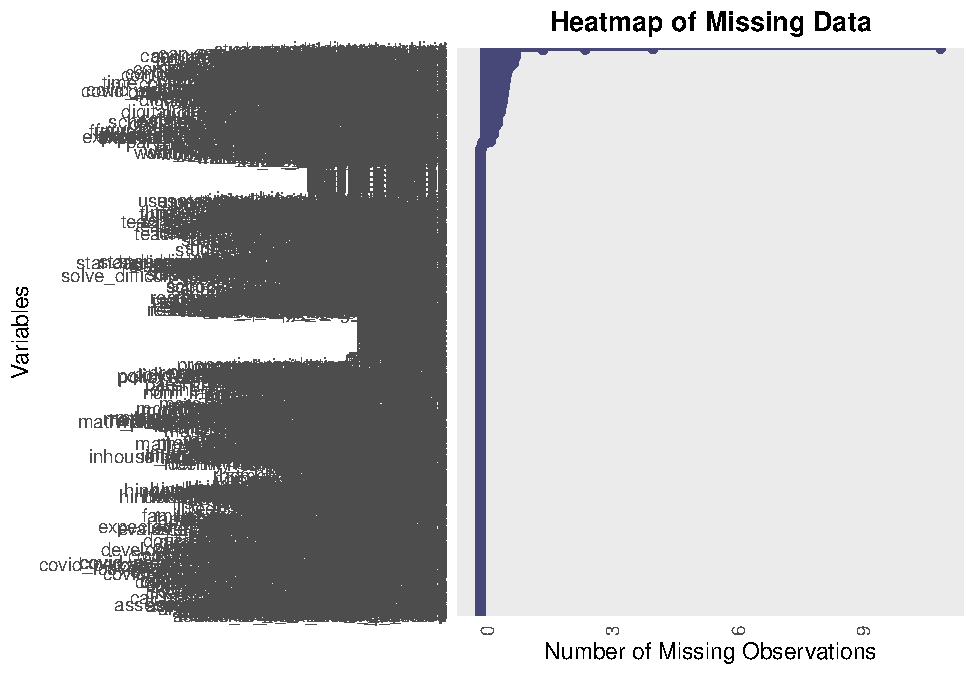
\includegraphics{PhD_Data_Analysis_files/figure-latex/missing_data_heatmap-1.pdf}

\textbf{Observations from the Heatmap:}

\textbf{1. No Variables with 100\% Missing Data}

The heatmap confirms that all variables with 100\% missingness have been
successfully excluded, as there are no columns entirely darkened.

\textbf{2. Patterns of Missingness}

Missing data appears concentrated in specific variables, with varying
intensities across the dataset. These patterns may indicate valid skips
or systematic differences that warrant further investigation.

\textbf{3. Subgroups of Interest}

Variables related to contextual factors, such as responses during
COVID-19 school closures, still exhibit moderate levels of missingness.
These missingness patterns likely correspond to valid skips (e.g.,
students whose schools remained open) and will be evaluated further in
the context of subgroup-specific analysis.

\textbf{4. Strategic Handling of Missingness}

Missing data mechanisms will be explored further to determine whether
subgroup-level patterns exist and whether missing values can be assumed
to be MCAR, MAR, or MNAR.

Depending on these findings, potential solutions may include subgroup
analysis, multiple imputation, or alternative statistical adjustments.

These insights guide the next step of categorizing missing data
mechanisms, allowing for targeted handling strategies.

\hypertarget{manual-addition-of-skip-logic-and-implications-of-skip}{%
\paragraph{Manual Addition of Skip Logic and Implications of
Skip}\label{manual-addition-of-skip-logic-and-implications-of-skip}}

Additional columns were created to further document and understand
missingness. The skip\_logic and implication\_of\_skip columns were
manually added to the response summary and populated based on relevant
documentation, including the PISA technical report and questionnaire
framework. This step ensures that decisions about inclusion/exclusion
are grounded in a complete understanding of missingness patterns and
their implications for analysis.

\textbf{1. Skip Logic}

The skip\_logic column records the administration pattern of each
variable. This includes whether a question was:

\begin{itemize}
\item
  Presented to All -- Administered to all students regardless of prior
  responses.
\item
  Randomized Subset -- Given to a subset of students selected through
  survey design.
\item
  Skip Based on Prior Response -- Administered conditionally based on
  earlier responses.
\end{itemize}

These assignments were based on PISA routing rules, response rates, and
the survey design framework.

\textbf{2. Implication of Skip}

The implication\_of\_skip column provides an interpretation of how skip
patterns affect data usability. Skipped responses may introduce
systematic missingness, meaning certain student groups may have higher
or lower response rates for specific questions. This column documents:

\begin{itemize}
\item
  Whether missingness is likely systematic (e.g., skipped due to a
  student's earlier response).
\item
  Whether the variable is only applicable to specific groups, which may
  limit generalizability.
\end{itemize}

Understanding how and why data are missing is essential for ensuring
methodologically sound handling of missingness. By explicitly
documenting skip logic and its implications, this step:

\begin{itemize}
\item
  Improves transparency in missing data assessment.
\item
  Helps refine inclusion/exclusion decisions by identifying variables
  with limited applicability.
\item
  Aligns the dataset with theoretical frameworks, ensuring analytical
  validity.
\end{itemize}

By systematically categorizing skip patterns and their impact, this
section lays the foundation for evaluating missing data mechanisms and
assessing potential redundancies or exclusions in the dataset.

\hypertarget{creation-of-status-columns-in-the-variable-mapping-table}{%
\paragraph{Creation of Status Columns in the Variable Mapping
Table}\label{creation-of-status-columns-in-the-variable-mapping-table}}

With initial assessment of missingness complete, status,
status\_priority, and status\_reason columns were created in the
variable mapping table. These columns document the provisional inclusion
status, theoretical priority, and rationale for each variable's
inclusion or exclusion.

\textbf{1. Assignment of Inclusion Status}

Each variable was assigned an inclusion status (Included or Excluded)
based on its alignment with research objectives, the PISA ICT Framework,
and the Multi-Level Framework of Technology Acceptance and Use (MLFTAU).
Additional practical considerations, such as missingness patterns and
survey design constraints, also informed these decisions.

\textbf{2. Determination of Priority Level}

To further differentiate variables by their theoretical and
methodological importance, a priority level was assigned in the
status\_priority column:

\begin{itemize}
\item
  High: Variables that are central to the research questions, directly
  aligned with theoretical models, and essential for key analyses.
\item
  Medium: Variables that contribute contextual insights or secondary
  analyses but are not strictly necessary for core research objectives.
\item
  Low: Variables that have limited theoretical significance or high
  levels of missingness, but may still provide exploratory value.
\end{itemize}

This priority ranking ensures that essential variables remain a focus of
the study while allowing flexibility for secondary and exploratory
analyses.

\textbf{3. Documentation of Rationale}

The rationale for each inclusion decision was documented in the
status\_reason column, providing clarity and transparency for all
decisions. This step ensures that each decision can be revisited and
understood in the context of the research.

\textbf{3. Integration with the Questionnaire Response Summary}

The status, priority level, and rationale columns from the updated
mapping table were then merged with the response summary file to update
the inclusion\_status, inclusion\_priority, and reason\_for\_decision
columns. This integration ensures consistency between the mapping table
and the response summary used in subsequent analysis.

\begin{Shaded}
\begin{Highlighting}[]
\CommentTok{\# Load necessary libraries}
\FunctionTok{library}\NormalTok{(dplyr)}
\FunctionTok{library}\NormalTok{(readr)}

\CommentTok{\# File paths}
\NormalTok{response\_summary\_path }\OtherTok{\textless{}{-}} \StringTok{"data/private/metadata/2022/pisa2022\_questionnaire\_response\_summary\_for\_missingness\_analysis.csv"}
\NormalTok{variable\_mapping\_path }\OtherTok{\textless{}{-}} \StringTok{"data/private/metadata/2022/pisa2022\_variable\_mapping\_table.csv"}

\CommentTok{\# Read files}
\NormalTok{response\_summary }\OtherTok{\textless{}{-}} \FunctionTok{read\_csv}\NormalTok{(response\_summary\_path)}
\NormalTok{variable\_mapping }\OtherTok{\textless{}{-}} \FunctionTok{read\_csv}\NormalTok{(variable\_mapping\_path)}

\CommentTok{\# Replace NAs with blank strings, except for specific columns}
\NormalTok{response\_summary }\OtherTok{\textless{}{-}}\NormalTok{ response\_summary }\SpecialCharTok{\%\textgreater{}\%}
  \FunctionTok{mutate}\NormalTok{(}\FunctionTok{across}\NormalTok{(}
    \SpecialCharTok{{-}}\FunctionTok{c}\NormalTok{(value, Label),  }\CommentTok{\# Exclude value and Label columns}
    \SpecialCharTok{\textasciitilde{}} \FunctionTok{ifelse}\NormalTok{(}\FunctionTok{is.na}\NormalTok{(.), }\StringTok{""}\NormalTok{, .)}
\NormalTok{  ))}

\CommentTok{\# Merge mapping table into response summary}
\NormalTok{response\_summary\_updated }\OtherTok{\textless{}{-}}\NormalTok{ response\_summary }\SpecialCharTok{\%\textgreater{}\%}
  \FunctionTok{left\_join}\NormalTok{(}
\NormalTok{    variable\_mapping }\SpecialCharTok{\%\textgreater{}\%}
      \FunctionTok{select}\NormalTok{(original\_variable\_name, status, status\_priority, status\_reason),}
    \AttributeTok{by =} \FunctionTok{c}\NormalTok{(}\StringTok{"original\_variable\_name"} \OtherTok{=} \StringTok{"original\_variable\_name"}\NormalTok{)}
\NormalTok{  ) }\SpecialCharTok{\%\textgreater{}\%}
  \FunctionTok{mutate}\NormalTok{(}
    \AttributeTok{inclusion\_status =} \FunctionTok{ifelse}\NormalTok{(}\FunctionTok{is.na}\NormalTok{(status), inclusion\_status, status),}
    \AttributeTok{inclusion\_priority =} \FunctionTok{ifelse}\NormalTok{(}\FunctionTok{is.na}\NormalTok{(status\_priority), inclusion\_priority, status\_priority),}
    \AttributeTok{reason\_for\_decision =} \FunctionTok{ifelse}\NormalTok{(}\FunctionTok{is.na}\NormalTok{(status\_reason), reason\_for\_decision, status\_reason)}
\NormalTok{  ) }\SpecialCharTok{\%\textgreater{}\%}
  \FunctionTok{select}\NormalTok{(}\SpecialCharTok{{-}}\NormalTok{status, }\SpecialCharTok{{-}}\NormalTok{status\_priority, }\SpecialCharTok{{-}}\NormalTok{status\_reason)}

\CommentTok{\# Save updated response summary}
\FunctionTok{write\_csv}\NormalTok{(response\_summary\_updated, response\_summary\_path)}

\FunctionTok{cat}\NormalTok{(}\StringTok{"Response summary successfully updated."}\NormalTok{)}
\end{Highlighting}
\end{Shaded}

\begin{Shaded}
\begin{Highlighting}[]
\CommentTok{\# Source the script for updating the response summary with status columns}
\CommentTok{\# This script automates the transformation and standardization of variables, while ensuring the resulting dataset remains proprietary and is used exclusively for academic research.}
\FunctionTok{source}\NormalTok{(}\StringTok{"scripts/2022/update\_response\_summary.R"}\NormalTok{)}
\end{Highlighting}
\end{Shaded}

\hypertarget{identification-and-removal-of-constant-variables}{%
\subsubsection{Identification and Removal of Constant
Variables}\label{identification-and-removal-of-constant-variables}}

To identify constant variables in the dataset, all variables with
identical values across all records were flagged. This process is
crucial because constant variables---those that do not provide variation
or meaningful information for analysis---can be removed to streamline
the dataset.

\textbf{Step 1: Creation of the Table of Constant Variables}

A table was created to isolate the variables with constant values. This
included variables such as country codes, sampling strata, and some
Weighted Likelihood Estimate (WLE) variables, which typically do not
exhibit variation across cases. These variables were reviewed to
determine if they were genuinely constant or if they provided critical
metadata that should be retained for future analyses.

The table below lists the identified constant variables, along with
their descriptions and constant values.

\begin{longtable}[t]{>{\raggedright\arraybackslash}p{2.5cm}>{\raggedright\arraybackslash}p{4.5cm}>{\raggedright\arraybackslash}p{6cm}>{\raggedright\arraybackslash}p{1.5cm}}
\caption{\label{tab:constant variables}Constant Variables Identified for Removal from the Dataset}\\
\toprule
Original Variable Name & Renamed Variable & Variable Description & Constant Value\\
\midrule
CNT & country\_code & Standard 3-character country code. & THA\\
CNTRYID & country\_id & Numerical identifier for countries; complements country\_code. & 764\\
CYC & assessment\_cycle & Identifies the PISA assessment cycle (e.g., 2022). & 08MS\\
NatCen & national\_center\_code & 6-character code for the national center coordinating the test. & 76400\\
STRATUM & sampling\_stratum & Sampling stratum used in PISA design for stratification. & THA97\\
\addlinespace
SUBNATIO & subnational\_region & Identifies subnational regions for analysis beyond national aggregates. & 7640000\\
OECD & oecd\_member & Binary indicator (1/0) for OECD membership. & 0\\
ADMINMODE & administration\_mode & Mode of test administration (e.g., computer- or paper-based). & 2\\
Option\_ICTQ & ict\_questionnaire\_flag & Indicates whether the student completed the ICT questionnaire. & 1\\
Option\_WBQ & well\_being\_flag & Indicates whether the student completed the well-being questionnaire. (Note: Not administered in Thailand) & 0\\
\addlinespace
Option\_PQ & parent\_questionnaire\_flag & Indicates whether the student’s parent completed the parent questionnaire. (Note: Not administered in Thailand) & 0\\
Option\_TQ & teacher\_questionnaire\_flag & Indicates whether the teacher completed the teacher questionnaire. (Note: Not administered in Thailand) & 0\\
Option\_UH & uh\_questionnaire\_flag & Indicates whether a school-level optional questionnaire was completed. (Note: Not administered in Thailand) & 0\\
ST006Q05JA & mother\_qualification\_4 & Whether the mother has a qualification at ISCED level 4. & 97\\
ST008Q05JA & father\_qualification\_4 & Whether the father has a qualification at ISCED level 4. & 97\\
\addlinespace
ST327Q04JA & expected\_complete\_qualification\_ISCED4 & Which of the following qualifications do you expect to complete: [ISCED level 4] & 97\\
PERSEVAGR & perseverance\_agreement & Agreement with perseverance statements. WLE variable reflecting persistence traits. & 97\\
COOPAGR & cooperation\_agreement & Agreement with cooperation statements. WLE variable measuring collaboration tendencies. & 97\\
EMPATAGR & empathy\_agreement & Agreement with empathy statements. WLE variable summarizing emotional understanding. & 97\\
ASSERAGR & assertiveness\_agreement & Agreement with assertiveness statements. WLE variable reflecting confidence. & 97\\
\addlinespace
STRESAGR & stress\_resistance\_agreement & Agreement with stress resistance statements. WLE variable measuring resilience. & 97\\
MATHEFF & math\_self\_efficacy & Mathematics self-efficacy for formal and applied tasks, with reversed response options in 2022. WLE variable reflecting confidence. & 97\\
FAMCON & math\_concept\_familiarity & Subjective familiarity with mathematics concepts. WLE variable measuring understanding. & 97\\
ANXMAT & math\_anxiety & Mathematics anxiety, measuring students' emotional responses to math. Derived using Weighted Likelihood Estimates (WLE). & 97\\
ICTENQ & ict\_enquiry\_learning & Use of ICT in enquiry-based learning activities. Calculated using WLE to represent active learning practices. & 97\\
\addlinespace
ICTFEED & ict\_support\_feedback & Support or feedback provided via ICT. A WLE variable summarizing teacher or peer support through technology. & 97\\
ICTOUT & ict\_outside\_class & Use of ICT for school-related activities outside the classroom. Derived using WLE. & 97\\
SC182Q10JA02 & math\_isc\_lvl5\_degree\_part & Part-time mathematics teachers with an ISCED Level 5 degree but not Level 6. & 0\\
DIGDVPOL & digital\_device\_policies & Weighted Likelihood Estimate (WLE) for digital device policies at the school & 97\\
DMCVIEWS & diversity\_multicultural\_views & Weighted Likelihood Estimate (WLE) for school diversity and multicultural views & 97\\
\bottomrule
\end{longtable}

\textbf{Step 2: Review and Decision Making}

After reviewing the table of constant variables, the decision was made
to retain certain variables, such as country\_code (CNT), country\_id
(CNTRYID), assessment\_cycle (CYC), and others, as they provide
essential metadata that are crucial for the structure of the dataset.

However, all excluded constant variables had a constant value of 97 (Not
Applicable) across all observations, meaning they contained no
meaningful variation and did not contribute any analytical value to the
research. Examples include:

\begin{itemize}
\item
  mother\_qualification\_4 (ST006Q05JA)
\item
  father\_qualification\_4 (ST008Q05JA)
\item
  Several Weighted Likelihood Estimate (WLE) variables
\end{itemize}

Since these variables provided no differentiation between observations,
they were removed from the dataset to reduce redundancy and improve
computational efficiency while ensuring the dataset remains
methodologically sound.

\textbf{Step 3: Deleting Constant Variables from the Dataset}

Following the decision to remove the identified constant variables, the
dataset was updated by deleting these variables from the data file
pisa2022\_cleaned\_4\_high\_missingness\_exclusion.csv to create a new
dataset, pisa2022\_cleaned\_5\_select\_constant\_variables\_removed.csv.

\begin{Shaded}
\begin{Highlighting}[]
\CommentTok{\# Source the script for removing select constant variables}
\CommentTok{\# This script automates the removal of select constant variables, while ensuring the resulting dataset remains proprietary and is used exclusively for academic research.}
\FunctionTok{source}\NormalTok{(}\StringTok{"scripts/2022/pisa2022\_cleaned\_5\_constant\_variable\_updates.R"}\NormalTok{)}
\end{Highlighting}
\end{Shaded}

\textbf{Step 4: Updating the Variable Mapping Table and Questionnaire
Response Summary}

The variable mapping table and questionnaire response summary were then
updated to reflect the exclusion of these constant variables. The
status, status\_priority, and status\_reason columns in the variable
mapping table were updated for the removed variables to indicate their
exclusion, with the reason stated as ``Constant variable''.

Similarly, the questionnaire response summary was updated by changing
the inclusion\_status, inclusion\_priority, and reason\_for\_decision
columns for these variables.

\begin{Shaded}
\begin{Highlighting}[]
\CommentTok{\# Source the script for updating inclusion/exclusion status of select constant variables}
\CommentTok{\# This script automates the updating of inclusion/exclusion status of select constant variables, while ensuring the resulting dataset remains proprietary and is used exclusively for academic research.}
\FunctionTok{source}\NormalTok{(}\StringTok{"scripts/2022/update\_inclusion\_exclusion\_status\_of\_select\_constant\_variables.R"}\NormalTok{)}
\end{Highlighting}
\end{Shaded}

This process of identifying and removing select constant variables,
along with the updates to the variable mapping table and response
summary, ensures that the dataset is both cleaner and more focused on
the relevant information for analysis.

\hypertarget{summary-and-next-steps-1}{%
\subsubsection{Summary and Next Steps}\label{summary-and-next-steps-1}}

The variable selection process for this study was methodically designed
to align with both theoretical frameworks and the research objectives.
The integration of the PISA Questionnaire Framework, PISA ICT Framework,
and the Multi-Level Framework of Technology Acceptance and Use (MLFTAU)
allowed for a comprehensive approach to variable identification. This
systematic method ensured that the selected variables reflect the
structural factors (such as ICT access) and measurable outcomes (like
ICT competencies) central to the study's aims.

During the variable selection process, several challenges were
encountered. Notably, the complexities of dual-labeling variables,
particularly those that spanned multiple constructs, required careful
attention to ensure accurate categorization without redundancy. The need
to maintain a balance between the expansive nature of the PISA ICT
Framework and the more behavioral, nuanced aspects of MLFTAU was another
area of focus. The ongoing task of ensuring empirical
suitability---given constraints like missing data---added an additional
layer of complexity. However, these challenges were effectively
addressed through iterative refinement and systematic mapping, ensuring
that all selected variables remained both theoretically relevant and
empirically suitable for the analysis.

With the variable selection process now complete, the next phase of the
study will focus on Data Preparation and Cleaning. This stage is
essential for transforming the raw dataset into a form suitable for
robust analysis. Key tasks in this phase include:

\begin{itemize}
\item
  Missing data will be handled by applying both granular techniques and
  imputation strategies to address gaps and ensure data completeness.
\item
  Ensuring consistency across datasets: To prepare for multi-cycle
  analysis, ensuring that the data from various years are harmonized to
  maintain comparability and consistency.
\end{itemize}

This preparatory work will provide a solid foundation for the following
stages of analysis, ensuring that the selected variables are not only
theoretically aligned but also ready for empirical investigation.

\hypertarget{handling-missing-data}{%
\subsection{Handling Missing Data}\label{handling-missing-data}}

\hypertarget{statistical-evaluation-of-missingness-patterns}{%
\subsubsection{Statistical Evaluation of Missingness
Patterns}\label{statistical-evaluation-of-missingness-patterns}}

Handling missing data is a critical step in this research to ensure the
validity and reliability of the findings. Missing data can introduce
bias, reduce statistical power, and affect the generalizability of
results, particularly in datasets with complex hierarchical structures
like PISA. Evaluating and addressing missingness is essential for
maintaining the integrity of the analysis and ensuring that the derived
conclusions accurately reflect the underlying phenomena.

The treatment of missing data requires a thorough understanding of its
nature and causes. Missing data can arise from various factors,
including survey design, non-response patterns, and data entry errors.
Left unaddressed, missingness can distort the relationships between
variables and compromise the comparability of results across different
groups or contexts. Consequently, careful consideration is given to
identifying, categorizing, and addressing missing data to preserve the
robustness and accuracy of the findings.

Evaluating missingness patterns in data is a crucial step in the data
preparation process, as it helps identify how and why data is missing.
Understanding the nature of the missingness (whether it is Missing
Completely at Random (MCAR), Missing at Random (MAR), or Missing Not at
Random (MNAR)) provides valuable insights into the integrity and
reliability of the dataset. This evaluation directly informs the
decisions made in subsequent steps of the analysis, particularly in how
missing data is handled. In earlier stages of the research process,
variables with high rates of missingness or constant values were
excluded, and the dataset was filtered for completeness and relevance.
However, the remaining missing data required careful consideration to
determine the most appropriate method for handling it.

\textbf{1. Imputation of Expected Education Level}

The variable expected\_education\_level serves as a key outcome variable
in this research, making the treatment of its missing values critical
for maintaining the validity and reliability of the analysis. An
evaluation of missingness patterns determined that the missing data
aligned with the Missing at Random (MAR) assumption, allowing for the
application of multiple imputation techniques.

Multiple Imputation by Chained Equations (MICE) was utilized to address
missing values, implemented through the mice package in R. This method
was selected due to its robustness and flexibility in handling MAR data
and its ability to incorporate auxiliary variables as predictors.

\begin{enumerate}
\def\labelenumi{\arabic{enumi}.}
\item
  Predictors were selected based on their correlation with
  expected\_education\_level and their theoretical relevance, including
  variables related to ICT use, socioeconomic status, and the school
  environment.
\item
  Five imputed datasets were generated, ensuring multiple plausible
  imputations. One completed dataset was selected for subsequent
  analysis to streamline the process and maintain consistency with the
  research workflow.
\item
  The distribution of imputed values was compared to observed data to
  verify plausibility, and convergence diagnostics were conducted to
  ensure stability across iterations.
\end{enumerate}

The final dataset
(pisa2022\_cleaned\_6\_imputed\_expected\_education\_level.csv) contains
the imputed values for expected\_education\_level alongside all other
original variables, with no changes made to the structure or values of
the dataset except for the imputed variable.

\begin{Shaded}
\begin{Highlighting}[]
\CommentTok{\# Source the script for imputing missing expected education level values}
\CommentTok{\# This script automates the process of multiple imputation using the MICE package,}
\CommentTok{\# while ensuring that only the variable \textasciigrave{}expected\_education\_level\textasciigrave{} is modified.}
\FunctionTok{source}\NormalTok{(}\StringTok{"scripts/2022/pisa2022\_cleaned\_6\_imputed\_expected\_education\_level.R"}\NormalTok{)}
\end{Highlighting}
\end{Shaded}

By incorporating the source script, this document provides a
reproducible link to the complete imputation process, ensuring
transparency and adherence to academic best practices.

\textbf{2. Recalculation of ICT Distress Online}

The ict\_distress\_online variable measures the level of distress
students experienced online when encountering inappropriate content,
discriminatory content, offensive messages, and the public dissemination
of personal information without consent. Given its importance in
analyzing students' digital experiences, ensuring its accurate
derivation is essential for meaningful analysis.

A review of the PISA 2022 dataset revealed that ict\_distress\_online
was derived as the sum of four input variables:

\begin{itemize}
\item
  upset\_inappropriate\_content
\item
  upset\_discriminatory\_content
\item
  upset\_offensive\_messages
\item
  upset\_info\_public\_without\_consent
\end{itemize}

While the methodology was broadly correct, a key issue was identified.
Students who selected ``This did not happen to me'' (1, 1, 1, 1) were
assigned \texttt{NA} instead of \texttt{0}, despite having valid
responses that indicated an absence of distress. Handling of 99 (``No
Response'') values was also reviewed and confirmed to follow PISA's
methodology, where valid responses were correctly summed while ignoring
99.

Therefore, a number of steps were taken to address this incorrect
handling of students who selected 1 (``This did not happen to me'') for
all four variables.

\begin{enumerate}
\def\labelenumi{\arabic{enumi}.}
\item
  In line with PISA methodology, the response scale was rescaled from
  1-5 to 0-4 to better reflect distress levels.
\item
  The original ict\_distress\_online variable was renamed
  ict\_distress\_online\_old to preserve its original values.
\item
  A new column ict\_distress\_online\_recalculated was created
  immediately after ict\_distress\_online\_old.
\item
  Students who selected 1,1,1,1 across all input variables were assigned
  a distress score of 0, rather than NA, ensuring that their responses
  were accurately reflected.
\item
  Cases where at least one response was coded as 99 were left unchanged,
  as these responses were already correctly handled by ignoring 99
  values and summing only valid responses.
\end{enumerate}

To verify the integrity of these changes, comparisons were conducted
between the original dataset (cleaned\_6) and the updated dataset
(cleaned\_7).

\begin{itemize}
\item
  The number of rows remained consistent.
\item
  The number or variables increased by one from 1115 to 1116, reflecting
  the addition of the ict\_distress\_online\_recalculated column.
\item
  The total count of missing (NA) values remained unchanged, confirming
  that no unintended modifications were introduced, since all NAs from
  ict\_distress\_online\_recalculated have been replaced by 0.
\item
  The count of 99 values increased slightly, reflecting the additional
  instances introduced in ict\_distress\_online\_recalculated.
\end{itemize}

The final dataset,
pisa2022\_cleaned\_7\_recalculated\_ict\_distress\_online.csv, now
ensures that students who did not experience distress are correctly
assigned a value of 0. This correction improves the accuracy and
reliability of analyses examining students' online experiences and
emotional well-being.

\begin{Shaded}
\begin{Highlighting}[]
\CommentTok{\# Source the script for recalculating the ICT distress online variable}
\CommentTok{\# This script ensures that the derived variable aligns with academic best practices }
\CommentTok{\# and the guidelines outlined in the PISA Technical Report.}
\FunctionTok{source}\NormalTok{(}\StringTok{"scripts/2022/pisa2022\_cleaned\_7\_recalculated\_ict\_distress\_online.R"}\NormalTok{)}
\end{Highlighting}
\end{Shaded}

\hypertarget{granular-handling-of-missing-data}{%
\subsubsection{Granular Handling of Missing
Data}\label{granular-handling-of-missing-data}}

A meticulous approach to handling missing data represents a critical
phase in this research, building upon the initial evaluation of
missingness patterns to address the specific characteristics of
variables within the dataset. While earlier stages excluded variables
with high missingness or constant values, this phase refines the dataset
further by systematically prioritizing variables, considering their
relevance, type, and role within the dataset. Special attention is given
to variables serving as inputs to derived constructs, ensuring that
decisions regarding inclusion or exclusion align with the research
objectives and the PISA framework.

The dataset encompasses diverse variables originating from the student
questionnaire (ST), ICT questionnaire (IC), school questionnaire (SC),
and derived indices provided by PISA. Each of these presents unique
considerations:

\begin{enumerate}
\def\labelenumi{\arabic{enumi}.}
\item
  Student and ICT Variables (ST and IC) are critical for assessing
  individual-level responses related to ICT use, behaviors, and
  attitudes.
\item
  School-Level Variables (SC) are aggregated data for all students in a
  school, offering contextual insights but less emphasis for
  individual-level analysis.
\item
  Derived Variables are precalculated indices such as plausible values
  (PVs) and composite indices essential for specific analyses but
  dependent on the quality and completeness of multiple input variables.
\end{enumerate}

This phase leverages the PISA 2022 Variable Mapping Table and the PISA
2022 Questionnaire Response Summary to systematically evaluate
variables. These resources enable the consistent classification,
validation, and prioritization of variables based on their relevance,
dependencies, and role in the analytical framework. By addressing these
elements, the granular handling process ensures that the dataset remains
robust, interpretable, and aligned with research objectives.

\hypertarget{prioritization-of-variables}{%
\paragraph{Prioritization of
Variables}\label{prioritization-of-variables}}

refines the dataset by systematically assessing and selecting variables
central to the research objectives, while accounting for dependencies on
derived constructs. This step uses the PISA 2022 Variable Mapping Table
to classify variables based on their relevance (high, medium, low) and
dependencies on derived variables, ensuring transparency and alignment
with methodological rigor.

Additionally, some PISA questionnaire responses are derived by
validating student responses against school questionnaire data or other
administrative sources. Furthermore, certain derived variables also act
as input variables for additional derived constructs, necessitating
careful documentation of these relationships.

\textbf{Classification by Relevance}

\begin{itemize}
\item
  High Relevance: Directly aligned with core constructs (e.g., ICT use,
  student well-being, or educational outcomes).
\item
  Medium Relevance: Provide contextual insights but are secondary to the
  primary research focus.
\item
  Low Relevance: Excluded unless critical to specific analyses or as
  input for derived constructs.
\end{itemize}

\textbf{Dependency on Derived Variables}

\begin{itemize}
\item
  Identification of variables that contribute to PISA-derived constructs
  such as plausible values (PVs), composite indices, and aggregated
  metrics.
\item
  Retention of all input variables and their associated derived
  constructs to preserve analytical integrity or exclusion of all if the
  derived variable is deemed non-essential.
\end{itemize}

\textbf{Updated Structure of the Variable Mapping Table}

To improve clarity and documentation of relationships between input
variables and derived constructs, new columns have been added to the
mapping table:

\begin{itemize}
\item
  derived\_variable (Yes/No): Indicates whether the variable is a
  derived construct.
\item
  derived\_variable\_calculation: The calculation logic for the derived
  construct, where available, or notes its absence.
\item
  derived\_variable\_validation: Indicates the validation status of the
  derived construct (e.g., ``Valid'' or ``Validation not feasible'').
  Invalid derived variables are corrected where possible, as was done
  previously with expected\_education\_level and ict\_online\_distress.
\item
  input\_variable (Yes/No): Identifies whether the variable is an input
  variable contributing to a derived construct.
\item
  dependent\_derived\_variable: Lists the derived constructs that rely
  on the input variable.
\end{itemize}

\textbf{Reevaluation of Inclusion/Exclusion}

Variables are systematically reviewed based on their relevance and role:

\begin{itemize}
\item
  High- and medium-relevance variables are prioritized.
\item
  Low-relevance variables are excluded unless serving critical roles in
  derived constructs.
\end{itemize}

By integrating these steps, the prioritization process ensures a focused
dataset that maintains the integrity of derived constructs while
aligning with the research's analytical framework.

After updating the status, status\_priority, and status\_reason columns
in the variable mapping table, the variables labeled as ``Excluded''
were systematically removed from the dataset to ensure that only
relevant variables are retained for the analysis.

This step is important for ensuring the dataset reflects the inclusion
decisions based on the status columns and the variable priority levels.
The variables marked as ``Excluded'' in the status column were removed
programmatically to prevent them from influencing subsequent analysis.

\begin{Shaded}
\begin{Highlighting}[]
\CommentTok{\# Load necessary libraries}
\FunctionTok{library}\NormalTok{(dplyr)}
\FunctionTok{library}\NormalTok{(readr)}

\CommentTok{\# Read in the cleaned dataset}
\NormalTok{pisa\_data\_cleaned\_4 }\OtherTok{\textless{}{-}} \FunctionTok{read.csv}\NormalTok{(}\StringTok{"data/private/processed/2022/pisa2022\_cleaned\_4\_high\_missingness\_exclusion.csv"}\NormalTok{)}

\CommentTok{\# Load the variable mapping table that identifies excluded variables}
\NormalTok{variable\_mapping\_table }\OtherTok{\textless{}{-}} \FunctionTok{read.csv}\NormalTok{(}\StringTok{"data/private/metadata/2022/pisa2022\_variable\_mapping\_table.csv"}\NormalTok{)}

\CommentTok{\# Identify excluded variables from the mapping table (filter by \textquotesingle{}Exclude\textquotesingle{} in \textquotesingle{}status\textquotesingle{} column)}
\NormalTok{excluded\_variables\_from\_mapping }\OtherTok{\textless{}{-}}\NormalTok{ variable\_mapping\_table }\SpecialCharTok{\%\textgreater{}\%}
  \FunctionTok{filter}\NormalTok{(status }\SpecialCharTok{==} \StringTok{"Excluded"}\NormalTok{) }\SpecialCharTok{\%\textgreater{}\%}
  \FunctionTok{select}\NormalTok{(renamed\_variable) }\SpecialCharTok{\%\textgreater{}\%}  \CommentTok{\# Updated to the correct column name}
  \FunctionTok{pull}\NormalTok{()  }\CommentTok{\# Extract the variable names as a vector}

\CommentTok{\# Check which excluded variables exist in the dataset}
\NormalTok{existing\_excluded\_vars }\OtherTok{\textless{}{-}}\NormalTok{ excluded\_variables\_from\_mapping[excluded\_variables\_from\_mapping }\SpecialCharTok{\%in\%} \FunctionTok{colnames}\NormalTok{(pisa\_data\_cleaned\_4)]}

\CommentTok{\# Get the number of excluded variables}
\NormalTok{num\_excluded\_variables }\OtherTok{\textless{}{-}} \FunctionTok{length}\NormalTok{(existing\_excluded\_vars)}

\CommentTok{\# Remove the excluded variables that exist in the dataset}
\NormalTok{pisa\_data\_cleaned\_5 }\OtherTok{\textless{}{-}}\NormalTok{ pisa\_data\_cleaned\_4 }\SpecialCharTok{\%\textgreater{}\%}
  \FunctionTok{select}\NormalTok{(}\SpecialCharTok{{-}}\FunctionTok{one\_of}\NormalTok{(existing\_excluded\_vars))}

\CommentTok{\# Get the number of remaining variables after exclusion}
\NormalTok{num\_remaining\_variables }\OtherTok{\textless{}{-}} \FunctionTok{ncol}\NormalTok{(pisa\_data\_cleaned\_5)}

\CommentTok{\# Save the intermediate cleaned dataset (after removing excluded variables) to a new file}
\FunctionTok{write.csv}\NormalTok{(pisa\_data\_cleaned\_5, }\StringTok{"data/private/processed/2022/pisa2022\_cleaned\_5\_logical\_exclusion.csv"}\NormalTok{, }\AttributeTok{row.names =} \ConstantTok{FALSE}\NormalTok{)}

\CommentTok{\# Confirm the removal and number of excluded variables}
\FunctionTok{cat}\NormalTok{(}\StringTok{"A total of"}\NormalTok{, num\_excluded\_variables, }\StringTok{"variables have been excluded from the dataset.}\SpecialCharTok{\textbackslash{}n}\StringTok{"}\NormalTok{)}
\FunctionTok{cat}\NormalTok{(}\StringTok{"The dataset has been saved as \textquotesingle{}pisa2022\_cleaned\_5\_logical\_exclusion.csv\textquotesingle{}.}\SpecialCharTok{\textbackslash{}n}\StringTok{"}\NormalTok{)}
\FunctionTok{cat}\NormalTok{(}\StringTok{"There are"}\NormalTok{, num\_remaining\_variables, }\StringTok{"variables remaining in the dataset after exclusion.}\SpecialCharTok{\textbackslash{}n}\StringTok{"}\NormalTok{)}
\end{Highlighting}
\end{Shaded}

\begin{Shaded}
\begin{Highlighting}[]
\CommentTok{\# Source the script for removing excluded variables}
\CommentTok{\# This script automates the removal of excluded variables, while ensuring the resulting dataset remains proprietary and is used exclusively for academic research.}
\FunctionTok{source}\NormalTok{(}\StringTok{"scripts/remove\_excluded\_variables.R"}\NormalTok{)}
\end{Highlighting}
\end{Shaded}

After running this code, the dataset
pisa2022\_cleaned\_5\_logical\_exclusion.csv is created, and all
variables marked as ``Excluded'' are removed from the dataset. The
confirmation output displays the number of variables excluded, as well
as the number of variables remaining in the dataset after exclusion. It
confirms that:

\begin{itemize}
\item
  A total of 86 variables are excluded
\item
  The dataset is saved as pisa2022\_cleaned\_5\_logical\_exclusion.csv
\item
  There are 1129 variables remaining in the dataset after exclusion.
\end{itemize}

Variables excluded during the status decision process remain in the
variable mapping table and questionnaire response summary. This decision
ensures transparency, facilitates reproducibility, and allows for
revisiting inclusion decisions in future research. Excluded variables
are programmatically filtered out during analysis to focus on the
included variables.

\hypertarget{treatment-of-missingness-by-variable-type}{%
\paragraph{Treatment of Missingness by Variable
Type}\label{treatment-of-missingness-by-variable-type}}

Student and ICT Variables (ST and IC): Handling NA, 95, 97, 98, and 99
values. Ensuring completeness for individual-level analyses.
School-Level Variables (SC): Addressing shared responses for students in
the same school. Minimizing bias in individual-level analyses. Derived
Variables: Validating precalculated indices (e.g., plausible values and
weights). Confirming consistency with PISA coding standards. Flagging
and addressing anomalies in derived indices.

\hypertarget{cross-referencing-summary-tables}{%
\paragraph{Cross-Referencing Summary
Tables}\label{cross-referencing-summary-tables}}

Leveraging the Student Response Summary Table for consistent treatment
of value codes and labels. Ensuring alignment with PISA-defined response
categories (e.g., 95, 97, 98, 99). Documenting decisions to preserve
transparency.

\hypertarget{identifying-and-handling-data-irregularities}{%
\paragraph{Identifying and Handling Data
Irregularities}\label{identifying-and-handling-data-irregularities}}

Detecting invalid, incomplete, or inconsistent responses. Strategies for
managing anomalies (e.g., imputation, exclusion, or categorization).
Discussion of thresholds for exclusion or further review.

\hypertarget{finalizing-the-dataset}{%
\paragraph{Finalizing the Dataset}\label{finalizing-the-dataset}}

Overview of changes made during granular handling. Summary of excluded
variables and rationale. Verification of dataset integrity (e.g., row
and column counts, checks for unintended changes).

\hypertarget{summary-and-next-steps-2}{%
\paragraph{Summary and Next Steps}\label{summary-and-next-steps-2}}

Brief recap of the granular handling process. Transition to subsequent
steps in data preparation (e.g., outlier detection, analytical
modeling).

\hypertarget{imputation-of-missing-data}{%
\subsubsection{Imputation of Missing
Data}\label{imputation-of-missing-data}}

\hypertarget{checking-for-redundancy}{%
\subsubsection{Checking for Redundancy}\label{checking-for-redundancy}}

To ensure parsimony and avoid multicollinearity in the dataset, this
study systematically identified and excluded redundant variables during
the selection process. Redundancy checks were critical in refining the
dataset for robust and interpretable statistical analysis, ensuring that
retained variables offered unique insights into ICT integration in
education.

Redundancy was assessed using both statistical and conceptual methods:

Statistical Screening Pairwise correlations among variables were
calculated to detect high correlations (greater than 0.85). This
threshold was chosen based on standard practices in multivariate
analysis, as variables with correlations above this value are considered
highly collinear and could distort the results of statistical models,
such as regression analyses.

For highly correlated pairs, the following approach was used:

Correlation Matrix: A correlation matrix was computed for the retained
variables to identify pairs of variables with high correlations.
Correlations above 0.85 were flagged as potentially redundant. Retention
Decision: For each pair of highly correlated variables, conceptual
alignment with the PISA ICT and MLFTAU frameworks was considered to
determine which variable to retain. The variable that provided the most
direct relevance to the research questions was kept, while the other was
excluded. Conceptual Alignment Beyond statistical measures, conceptual
redundancy was assessed by reviewing the variables for overlap in what
they measured, especially when indicators were highly similar within a
framework or across frameworks. For example, variables that measure
similar dimensions of ICT access (e.g., internet access at home
vs.~internet access at school) might be conceptually redundant.

The review process involved:

Framework Review: Each pair of highly correlated variables was reviewed
within the context of the PISA ICT and MLFTAU frameworks. The goal was
to retain the variable that best aligned with the research objectives
and provided unique insights into ICT integration in education.
Relevance to Research Objectives: The retained variable was chosen based
on its ability to address the research objectives clearly and
comprehensively, ensuring it added value to the analysis without
duplicating information from other variables. Example of Redundancy
Check: For example, consider two variables that measure ICT access:

Access to ICT at Home and Access to ICT at School. Although both are
related to ICT access, they capture slightly different dimensions (one
is home-based, the other school-based). However, if both variables are
highly correlated, the decision would be made based on the conceptual
alignment with the framework. If the study focuses on home-based
learning, Access to ICT at Home might be retained, while the other would
be excluded.

Variables were excluded if:

\begin{itemize}
\item
  They exhibited a high correlation (\textgreater{} 0.85) with another
  variable measuring the same construct.
\item
  Their theoretical alignment was weaker compared to alternatives
  measuring the same phenomenon.
\item
  Their inclusion introduced redundancy without adding actionable
  insights.
\end{itemize}

For instance, the variables capturing teacher training for ICT
integration (e.g., ``Teacher ICT Training Frequency'' and ``Teacher ICT
Confidence Levels'') exhibited redundancy. The variable ``Teacher ICT
Confidence Levels'' was retained due to its stronger alignment with both
behavioral constructs in MLFTAU and process dimensions in the PISA ICT
Framework.

Following redundancy checks, a total of X variables were excluded,
leaving Y unique variables aligned with the research frameworks. This
streamlined dataset ensures that each variable contributes distinct
value to the analysis, supporting robust and actionable findings.

\hypertarget{summary-and-next-steps-3}{%
\subsubsection{Summary and Next Steps}\label{summary-and-next-steps-3}}

\hypertarget{outlier-detection-and-treatment}{%
\subsection{Outlier Detection and
Treatment}\label{outlier-detection-and-treatment}}

Define what constitutes an outlier in the context of the PISA dataset.
Emphasize their potential impact on analyses, such as distorting means,
variances, and regression estimates. Highlight the importance of
identifying and handling outliers for the study's validity. Outlier
Detection Methods

Describe the methods used to identify outliers: Univariate Outliers: Use
thresholds like z-scores, interquartile range (IQR), or domain-specific
thresholds to flag extreme values in individual variables. Multivariate
Outliers: Use techniques like Mahalanobis distance to identify unusual
combinations of values across variables. Contextual Outliers: Consider
contextual factors, such as school-level averages that are extreme
compared to other schools. Handling Outliers

Outline strategies for handling outliers, such as: Retaining outliers
that are valid but extreme responses. Transforming or winsorizing
extreme values to reduce their impact. Removing outliers that represent
clear errors or invalid entries. Highlight how decisions about outliers
will depend on their context and the research objectives.
Cross-Referencing Other Sections

Note overlaps with earlier processes (e.g., the recalculation of
variables like ICT distress online may also reveal outliers).
Cross-reference sections where outliers could significantly affect
imputation or aggregated indices. Outputs and Verification

Document the flagged and handled outliers in a log file. Summarize the
number of outliers identified and the steps taken to handle them.

Summary and Next Steps

\hypertarget{analytical-methods}{%
\subsection{Analytical Methods}\label{analytical-methods}}

In the example analysis below, the plausible values and weight for the
specified year are accessed from the lists, and the average mathematics
performance is calculated by gender, demonstrating the practical use of
the data and lists.

\textbf{Handling of Plausible Values (PVs) and Weights}

The PISA dataset includes Plausible Values (PVs) for student achievement
scores in reading, mathematics, science, and creative thinking. PVs are
multiple imputed estimates of students' latent abilities rather than
exact scores, which means they are essential for accurate statistical
inferences and valid comparisons across student groups. Unlike single
point estimates, PVs account for measurement error by providing a range
of estimates, enhancing the validity of inferences drawn from these
scores. For this study, PVs will be applied in all analyses involving
student performance, aligning with best practices in large-scale
assessments to ensure robust statistical conclusions.

Additionally, survey weights are provided in the PISA dataset to adjust
for the complex sampling designs used, ensuring the sample accurately
represents the broader population. Since PISA employs stratified
sampling to capture diverse student populations, applying these weights
corrects for selection probability differences, allowing for
generalizable and unbiased parameter estimates. Weights are particularly
critical in maintaining statistical rigor in this study, as they ensure
that results are representative of Thailand's student population. In all
analyses involving PVs, the corresponding survey weights will be applied
to control for sampling biases and uphold the validity of statistical
inferences.

A range of statistical techniques will be applied to analyze the data.

Descriptive Statistics: To provide an overview of key variables related
to ICT use and student performance.

Hierarchical Linear Modeling (HLM): This technique will be used to
account for the nested structure of the PISA data (students within
schools). HLM models will help analyze the relationships between ICT
access, school characteristics, and student performance.

Weighted Linear Regression: This will assess the impact of ICT use on
student outcomes while accounting for the survey's sampling design.

Plausible Values (PVs): PVs will be used to represent student
performance across multiple dimensions, accounting for uncertainty in
test scores. The EdSurvey package will be utilized to handle PVs in
analysis.

\hypertarget{model-validation}{%
\subsection{Model Validation}\label{model-validation}}

Validation techniques, such as cross-validation and sensitivity
analysis, will be employed to ensure the robustness of the models. This
includes testing for assumptions, identifying potential biases, and
assessing model stability.

\hypertarget{addressing-validity-and-reliability}{%
\section{Addressing Validity and
Reliability}\label{addressing-validity-and-reliability}}

The study ensures both validity and reliability through carefully
designed data handling procedures, the use of well-established data
sources, and robust analytical techniques. Several strategies are
employed to maintain the highest standards of academic rigor:

\hypertarget{validity}{%
\subsection{Validity}\label{validity}}

Content Validity: The selection of variables is closely aligned with the
CIPO model and the Multi-Level Framework of Technology Acceptance and
Use (MLFTAU), ensuring that the constructs being measured accurately
reflect the key dimensions of ICT integration and educational outcomes.

Construct Validity: All key variables, such as ICT access, ICT
utilization, and student performance, are derived from reliable and
validated instruments within the PISA datasets and national databases,
providing confidence that these constructs are measured as intended.

Internal Validity: Potential confounding variables (e.g., socio-economic
status, school infrastructure) are controlled for using appropriate
statistical techniques such as Hierarchical Linear Modeling (HLM) and
weighted regression, minimizing the impact of extraneous factors on the
results.

External Validity: The use of national-level PISA data and a
well-defined sampling framework ensures that findings are generalizable
to the broader population of Thai students and schools, as well as
potentially applicable to other contexts with similar educational
environments.

\hypertarget{reliability}{%
\subsection{Reliability}\label{reliability}}

Measurement Reliability: The PISA dataset, along with other national
data sources, undergoes thorough validation and testing to ensure
consistency and accuracy in the measurement of variables. The use of
Plausible Values (PVs) further strengthens reliability by accounting for
the uncertainty inherent in student performance data.

Reproducibility: All steps of the analysis are fully documented in this
RMarkdown document, ensuring that the code, data processing steps, and
statistical analyses are transparent and reproducible. This includes the
use of the EdSurvey package to manage the complex sampling design and
PVs, ensuring that future researchers can replicate the analysis.

Analytical Techniques: Established statistical methods (e.g., HLM,
weighted linear regression) are applied rigorously, with models
validated through techniques such as cross-validation and sensitivity
analysis to check for consistency and robustness.

\hypertarget{documentation-and-transparency}{%
\subsection{Documentation and
Transparency}\label{documentation-and-transparency}}

All R code, data manipulations, and analysis steps are documented in
this RMarkdown file, ensuring that the research process is transparent
and easily replicable by others. The document adheres to best practices
for reproducible research, including version control through GitHub,
ensuring that any future updates or revisions are traceable.

By maintaining strict adherence to these principles, the study produces
results that are both accurate and generalizable, with confidence in the
reliability and validity of the findings. The combination of robust data
sources, appropriate statistical techniques, and clear documentation
ensures the integrity and reproducibility of the research.

\hypertarget{ethical-considerations}{%
\section{Ethical Considerations}\label{ethical-considerations}}

This research adheres to the highest standards of ethical conduct as
outlined by international and institutional guidelines for research
involving human data. Several key ethical principles guide the study to
ensure respect for individuals, data confidentiality, and the broader
sociocultural context:

\hypertarget{data-confidentiality-and-privacy}{%
\subsection{Data Confidentiality and
Privacy}\label{data-confidentiality-and-privacy}}

The data used in this study, including individual-level PISA data, are
anonymized to protect the identity and privacy of students and schools.
No personally identifiable information (PII) is used in the analysis,
and data are handled in accordance with national and international data
protection regulations (e.g., GDPR where applicable).

Strict access control measures are in place to ensure that the data is
only accessed by authorized personnel for the purposes of this research.
The dataset is stored securely, and all analyses are conducted in a
manner that prevents the identification of individual respondents.

The use of Plausible Values (PVs) in the PISA dataset enhances privacy
by ensuring that no single score can be directly attributed to a
specific student, thereby preserving confidentiality.

\hypertarget{transparency-and-honesty-in-reporting}{%
\subsection{Transparency and Honesty in
Reporting}\label{transparency-and-honesty-in-reporting}}

All findings are reported accurately and without manipulation or bias.
The methodology is fully transparent, allowing for the reproducibility
and scrutiny of results. Potential limitations or biases in the data are
acknowledged and addressed, ensuring that the findings contribute
meaningfully to both academic knowledge and policy discussions.

In line with best practices, the study commits to sharing anonymized
data, code, and methodology transparently via platforms such as GitHub,
allowing for peer review and replicability of the research.

\hypertarget{respect-for-sociocultural-context}{%
\subsection{Respect for Sociocultural
Context}\label{respect-for-sociocultural-context}}

The study recognizes the importance of Thailand's unique sociocultural
and educational landscape. Special attention is paid to ensuring that
the research does not reinforce inequities or biases inherent in the
data, particularly with respect to disadvantaged and marginalized
groups.

Ethical considerations include the contextual sensitivity of findings,
ensuring that policy recommendations are culturally appropriate and do
not disproportionately disadvantage any group. The study aims to
contribute positively to the development of Thailand's education system
by offering evidence-based, inclusive policy suggestions.

\hypertarget{compliance-with-ethical-review-boards}{%
\subsection{Compliance with Ethical Review
Boards}\label{compliance-with-ethical-review-boards}}

The study has been reviewed and approved by the Internal Review Board
(IRB) of the researcher's institution, ensuring that it meets ethical
standards regarding data use, privacy, and the handling of sensitive
information.

In line with institutional and international ethical guidelines (e.g.,
APA and the Declaration of Helsinki), the research adheres to principles
of respect for persons, beneficence, and justice, ensuring that all
steps in the research process protect the dignity and rights of
individuals represented in the data.

\hypertarget{policy-and-societal-implications}{%
\subsection{Policy and Societal
Implications:}\label{policy-and-societal-implications}}

The study is designed with careful consideration of its potential policy
implications. Recommendations made as a result of the findings aim to
improve educational outcomes in Thailand and to close the digital
divide, particularly for marginalized communities. Ethical
responsibility is taken to ensure that these recommendations are
grounded in evidence and are not used in ways that could negatively
impact vulnerable populations.

By adhering to these ethical principles, the research not only ensures
compliance with data protection and privacy standards but also
contributes positively to educational policy and practice in Thailand in
a responsible and culturally sensitive manner.

\end{document}
